
%  Beamer Style
\documentclass[xcolor={dvipsnames,rgb}]{beamer}

% \usepackage{enumitem}
%\includeonlyframes{current}
% \includeonlyframes{semantics,semantics2}

\usepackage{appendixnumberbeamer}

\usepackage{lmodern}
\usepackage[utf8]{inputenc}
\relax% Beamer Theme Customization...
    % \usetheme{default}
    \usetheme{Boadilla}
    % \ProcessOptionsBeamer
    % \useinnertheme[shadow]{rounded}
    \setbeamertemplate{blocks}[rounded][shadow=false]

    \setbeamertemplate{footline}
    {
      \leavevmode%
      \hbox{%
      \begin{beamercolorbox}[wd=.3\paperwidth,ht=2.25ex,dp=1ex,center]{author in head/foot}%
        \usebeamerfont{author in head/foot}\insertshortauthor
      \end{beamercolorbox}%
      \begin{beamercolorbox}[wd=.6\paperwidth,ht=2.25ex,dp=1ex,center]{title in head/foot}%
        \usebeamerfont{title in head/foot}\insertshorttitle
      \end{beamercolorbox}%
      \begin{beamercolorbox}[wd=.1\paperwidth,ht=2.25ex,dp=1ex,center]{date in head/foot}%
        \insertframenumber{} / \inserttotalframenumber\hspace*{1ex}
      \end{beamercolorbox}}%
      \vskip0pt%
    }

	\setbeamersize{description width=0.57cm}
	\usefonttheme[stillsansserifsmall]{serif}
		% \usefonttheme{structuresmallcapsserif}
	\usefonttheme[onlylarge]{structuresmallcapsserif}
		% \usefonttheme[onlymath]{serif}
		% \usefonttheme[onlysmall]{structurebold}
	\setbeamerfont{item}{series=\bfseries}
    \setbeamerfont{subsection in toc}{size=\small}
		% \setbeamerfont{section in toc}{size=\normalsize,series=\bfseries,shape=\upshape}
		\setbeamerfont{section in toc}{size=\normalsize}
	\setbeamerfont{block title}{series=\bfseries}
	% \setbeamerfont{title}{family=\rmfamily}

	\relax%%% color definitions %%...
		\colorlet{structurecolor}{RoyalPurple!50!black}
		\colorlet{alertcolor}{YellowOrange}
			% \colorlet{alertcolor}{structurecolor>wheel,1,3}
		\colorlet{benchcolor1}{Emerald!85!black}
			% \colorlet{benchcolor1}{structurecolor>wheel,2,3}
		\colorlet{benchcolor2}{YellowOrange!25!magenta}
	\usecolortheme[named=structurecolor]{structure}
		% \usecolortheme{beaver}
		% \setbeamercolor*{palette primary}{bg=color1, fg = green}
		% \setbeamercolor*{palette secondary}{bg=color2, fg = green}
		% \setbeamercolor*{palette tertiary}{bg=color3, fg = green}
		% \setbeamercolor*{palette quaternary}{bg=color4, fg = green}
		% \makeatletter
		% \definecolor{beamer@blendedblue}{rgb}{0.2,0.2,0.7}
		% \colorlet{beamer@blendedblue}{color2}
		% \makeatother
	\setbeamercolor{description item}{bg={structurecolor!20!white}}
	% \setbeamercolor{alerted text}{fg=alertcolor!85!red}
	\setbeamercolor{alerted text}{fg=alertcolor}
	\gdef\customnav{}
  % \setbeamertemplate{navigation symbols}{\customnav\insertframenavigationsymbol}
  \setbeamertemplate{navigation symbols}{\customnav~\insertsectionnavigationsymbol}
	\setbeamercolor{button}{fg=structurecolor,bg=structurecolor!15!white}
	\renewcommand\beamerreturnbutton[1]{{%
			\setbeamercolor{button}{fg=structurecolor!15!white,bg=black}%
			\beamerbutton{\insertreturnsymbol#1}%
		}}

  \makeatletter
  \newlength\beamerleftmargin
  \setlength\beamerleftmargin{\Gm@lmargin}
  %% stolen from:
  % https://tex.stackexchange.com/questions/34458/reference-overlay-numbers-with-names
  \DeclareRobustCommand*{\savepause}[1]{\only<1>{\immediate\write\@auxout{\string\pauseentry{\the\c@framenumber}{#1}{\the\c@beamerpauses}}}}
  \newcommand*{\usepause}[1]{\@ifundefined{pauses@\the\c@framenumber @#1}{1}{\@nameuse{pauses@\the\c@framenumber @#1}}}
  \newcommand*{\pauseentry}[3]{\global\@namedef{pauses@#1@#2}{#3}}
  \makeatother

  \newbool{precompiledfigs}% ...
	\setbool{precompiledfigs}{false}
		% the etoolbox way, which works with beamer.
	% \setbeamercovered{dynamic}

\relax %%%%%%%%  Beamer and slide-specific macros  %%%%%%%%%%%%%%%%%%%
	\newcommand<>{\hl}[2][alertcolor]{\begingroup%
		\setbeamercolor{alerted text}{fg=#1}\alert#3{#2}\endgroup}
	\colorlet{notationcolor}{structurecolor!30}
	\colorlet{notationalertedcolor}{structurecolor!20!alertcolor!40}
    \setbeamercolor{base notation}{fg=notationcolor}
    \setbeamercolor{alerted notation}{fg=notationalertedcolor}
	% \def\notation#1{\!\hl[notationcolor]{#1$\quad$}}
    \setbeamertemplate{alerted text begin}{
        % Set the notation color to alerted notation
        \setbeamercolor{notation}{use={alerted notation},%
            fg=alerted notation.fg,bg=alerted notation.bg}%
        %... and set the local structure to alerted text.
        \setbeamercolor{local structure}{use={alerted text},%
            fg=alerted text.fg,bg=alerted text.bg}}
    \setbeamertemplate{alerted text end}{%
        % probably no need to reset, because dying scope will reset the notation color.
        % \setbeamercolor{notation}{fg=base notation.fg, bg=base notation.bg}
    }
    % \setbeamercolor{notation}{parent={alerted text,normal text}}
	\newcommand{\notation}[1]{%
        {\usebeamercolor{notation}%
        \!\color{fg}#1$\quad$}}

	% \newcommand<>{\alertwith}[2]{\begingroup\only#3{\setbeamercolor{alerted text}{fg=#1}}#2\endgroup} % DOESN'T WORK THIS WAY
	\newenvironment{localfocusenv}{\only{\setbeamercolor{local structure}{fg=alertcolor}}}{}
	% \newenvironment<>{hidemeenv}{%
	% 	\only#1{\setbeamercolor{alerted text}{fg=black!60}}%
	% 	\begingroup\begin{alertenv}#1%
	% 	}{\end{alertenv}\endgroup}
	\newenvironment<>{hidemeenv}{%
        \begingroup\only#1{%
        %     \setbeamercolor{alerted text}{use={alerted text,background canvas},%
        %         fg=alerted text.fg!30!background canvas.bg}%
            \setbeamercolor{faded text}{%use={background canvas},%
                fg=normal text.fg!25!background canvas.bg}%
            \setbeamercolor{local structure}{use={faded text},fg=faded text.fg}%
            \setbeamercolor{notation}{use={base notation},fg=base notation.fg!40!background canvas.bg}
            \setbeamercolor{alerted notation}{fg=notationalertedcolor!30!background canvas.bg}
            \usebeamercolor[fg]{faded text}
        }}{\endgroup}
    \newenvironment<>{catblock}[1]{%
      \setbeamercolor{block title}{fg=white,bg=blue!95!black}
      \setbeamercolor{block body}{fg=white,bg=black}
      \begin{block}#2{#1}}{\end{block}}

	\newenvironment<>{tikzpicture||precompiled}[2][]{
			\ifbool{precompiledfigs}{\includegraphics[width=0.8\linewidth]{figure-pdfs/#2}
				}\begingroup\only#3\begingroup\begin{tikzpicture}[#1]
		}{\end{tikzpicture}\endgroup\endgroup}
	\newcommand<>{\extra}[2][]{%
		\only#3{%
			% \tikzmark{call point};%
			\tikzro \node[inner sep=0pt,outer sep=0pt] (call point) {};%
			\begin{tikzpicture}[overlay,remember picture]
				\node[anchor=north west, inner sep=0.8em,
				 			fill=alertcolor!30!structurecolor!30!white,
							draw=structurecolor!70!black, draw opacity=0.5,
							below=1em of call point, #1]{#2};
			\end{tikzpicture}%
		}}
	\newcommand{\tikzro}[1][]{\tikz[remember picture, overlay,#1]}
	\def\Set{\mathbf{Set}}
	% "light gray script script"
	\def\lgss{\color{gray!80}\scriptscriptstyle}%
	\makeatletter
	\newcommand{\shorteq}{%
	  \settowidth{\@tempdima}{-}% Width of hyphen
	  \resizebox{\@tempdima}{\height}{=}%
	}
	\makeatother
    %https://tex.stackexchange.com/questions/34921/how-to-overlap-images-in-a-beamer-slide
    \def\Put(#1,#2)#3{\leavevmode\makebox(0,0){\put(#1,#2){#3}}}

	% \newcommand{\tikzmark}[1][last mark]{\tikzro \node (#1){};}

\usepackage{tikz} % Tikz + Tikz Customization 
	\usetikzlibrary{positioning,calc, arrows, shapes}

	\tikzset{AmpRep/.style={ampersand replacement=\&}}
	\tikzset{center base/.style={baseline={([yshift=-.8ex]current bounding box.center)}}}
	\tikzset{paperfig/.style={center base,scale=0.9, every node/.style={transform shape}}}

	\tikzset{dpadded/.style={rounded corners=2, inner sep=0.6em, draw, outer sep=0.2em, fill={black!50}, fill opacity=0.08, text opacity=1}}
	\tikzset{light pad/.style={outer sep=0.2em, inner sep=0.5em, draw=gray!50}}
	\tikzset{arr/.style={draw, ->, thick, shorten <=3pt, shorten >=3pt}}
	\tikzset{arr0/.style={draw, ->, thick, shorten <=0pt, shorten >=0pt}}
	\tikzset{arr1/.style={draw, ->, thick, shorten <=1pt, shorten >=1pt}}
	\tikzset{arr2/.style={draw, ->, thick, shorten <=2pt, shorten >=2pt}}

	\newcommand{\drawbb}%
		{\draw (current bounding box.south west) rectangle (current bounding box.north east);}
	\ifbool{precompiledfigs}{}{
		\usetikzlibrary{fit, decorations,shapes.geometric}
		\usetikzlibrary{tikzmark}
		\usetikzlibrary{backgrounds}
		\pgfdeclarelayer{foreground}
		\pgfsetlayers{background,main,foreground}

		\pgfdeclaredecoration{arrows}{draw}{
			\state{draw}[width=\pgfdecoratedinputsegmentlength]{%
				\path [every arrow subpath/.try] \pgfextra{%
					\pgfpathmoveto{\pgfpointdecoratedinputsegmentfirst}%
					\pgfpathlineto{\pgfpointdecoratedinputsegmentlast}%
				};
		}}

		% \tikzset{dpad0/.style={outer sep=0.05em, inner sep=0.3em, draw=gray!75, rounded corners=4, fill=black!08, fill opacity=1}}
		\tikzset{dpad0/.style={outer sep=0.05em, inner sep=0.2em, draw=gray!75, draw opacity=0.5, rounded corners=3, fill=black!18, fill opacity=0.4, text=black, text opacity=1}}

		\tikzset{dpad/.style args={#1}{every matrix/.append style={nodes={dpadded, #1}}}}
		\tikzset{is bn/.style={background rectangle/.style={fill=blue!35,opacity=0.3, rounded corners=5},show background rectangle}}
		% \usetikzlibrary{backgrounds}
		% \usetikzlibrary{patterns}
		\usetikzlibrary{cd}

		\tikzset{fgnode/.style={dpadded,inner sep=0.2em, circle,minimum width=2.3em},
				 factor/.style={light pad, fill=black, outer sep=0pt,draw=none}}


		\newcommand\cmergearr[5][]{
			\draw[arr, #1, -] (#2) -- (#5) -- (#3);
			\draw[arr, shorten <=0, #1] (#5) -- (#4);
			}
		\newcommand\mergearr[4][]{
			\coordinate (center-#2#3#4) at (barycentric cs:#2=1,#3=1,#4=1.2);
			\cmergearr[#1]{#2}{#3}{#4}{center-#2#3#4}
			}
		\newcommand\cunmergearr[5][]{
			\draw[arr, #1, -, shorten >=0] (#2) -- (#5);
			\draw[arr, shorten <=0, #1] (#5) -- (#3);
			\draw[arr, shorten <=0, #1] (#5) -- (#4);
			}
		\newcommand\unmergearr[4][]{
			\coordinate (center-#2#3#4) at (barycentric cs:#2=1.2,#3=1,#4=1);
			\cunmergearr[#1]{#2}{#3}{#4}{center-#2#3#4}
			}


		\usetikzlibrary{matrix}
		\tikzset{toprule/.style={%
		        execute at end cell={%
		            \draw [line cap=rect,#1]
		            (\tikzmatrixname-\the\pgfmatrixcurrentrow-\the\pgfmatrixcurrentcolumn.north west) -- (\tikzmatrixname-\the\pgfmatrixcurrentrow-\the\pgfmatrixcurrentcolumn.north east);%
		        }
		    },
		    bottomrule/.style={%
		        execute at end cell={%
		            \draw [line cap=rect,#1] (\tikzmatrixname-\the\pgfmatrixcurrentrow-\the\pgfmatrixcurrentcolumn.south west) -- (\tikzmatrixname-\the\pgfmatrixcurrentrow-\the\pgfmatrixcurrentcolumn.south east);%
		        }
		    },
		    leftrule/.style={%
		        execute at end cell={%
		            \draw [line cap=rect,#1] (\tikzmatrixname-\the\pgfmatrixcurrentrow-\the\pgfmatrixcurrentcolumn.north west) -- (\tikzmatrixname-\the\pgfmatrixcurrentrow-\the\pgfmatrixcurrentcolumn.south west);%
		        }
		    },
		    rightrule/.style={%
		        execute at end cell={%
		            \draw [line cap=rect,#1] (\tikzmatrixname-\the\pgfmatrixcurrentrow-\the\pgfmatrixcurrentcolumn.north east) -- (\tikzmatrixname-\the\pgfmatrixcurrentrow-\the\pgfmatrixcurrentcolumn.south east);%
		        }
		    },
		    table with head/.style={
			    matrix of nodes,
			    row sep=-\pgflinewidth,
			    column sep=-\pgflinewidth,
			    nodes={rectangle,minimum width=2.5em, outer sep=0pt},
			    row 1/.style={toprule=thick, bottomrule},
	  	    }
			}
		\usepackage{environ}
\usepackage{xstring}

% Wow this works I'm brilliant
\def\wrapwith#1[#2;#3]{
	\expandarg\IfSubStr{#1}{,}{
		\expandafter#2{\expandarg\StrBefore{#1}{,}}
		\expandarg\StrBehind{#1}{,}[\tmp]
		\xdef\tmp{\expandafter\unexpanded\expandafter{\tmp}}
		#3
		\wrapwith{\tmp}[#2;{#3}]
	}{ \expandafter#2{#1} }
}
\def\hwrapcells#1[#2]{\wrapwith#1[#2;&]}
\def\vwrapcells#1[#2]{\wrapwith#1[#2;\\]}
\NewEnviron{mymathenv}{$\BODY$}

\newcommand{\smalltext}[1]{\text{\footnotesize#1}}
\newsavebox{\idxmatsavebox}
\def\makeinvisibleidxstyle#1#2{\phantom{\hbox{#1#2}}}
\newenvironment{idxmatphant}[4][\color{gray}\smalltext]{%
	\def\idxstyle{#1}
	\def\colitems{#3}
	\def\rowitems{#2}
	\def\phantitems{#4}
	\begin{lrbox}{\idxmatsavebox}$%$\begin{mymathenv}
	\begin{matrix}  \begin{matrix} \hwrapcells{\colitems}[\idxstyle]  \end{matrix}
		% &\vphantom{\idxstyle\colitems}
		\\[-0.05em]
		\left[
		\begin{matrix}
			\hwrapcells{\phantitems}[\expandafter\makeinvisibleidxstyle\idxstyle]  \\[-1.2em]
	}{
		\end{matrix}\right]		&\hspace{-0.8em}\begin{matrix*}[l] \vwrapcells{\rowitems}[\idxstyle] \end{matrix*}\hspace{0.1em}%
	\end{matrix}%
	$%\end{mymathenv}
	\end{lrbox}%
	\raisebox{0.75em}{\usebox\idxmatsavebox}
%	\vspace{-0.5em}
}

\newenvironment{idxmat}[3][\color{gray}\smalltext]
	{\begingroup\idxmatphant[#1]{#2}{#3}{#3}}
	{\endidxmatphant\endgroup}

\newenvironment{sqidxmat}[2][\color{gray}\smalltext]
	{\begingroup\idxmat[#1]{#2}{#2}}
	{\endidxmat\endgroup}


%%%%%%%%%%%%
% better alignment for cases
\makeatletter
\renewenvironment{cases}[1][l]{\matrix@check\cases\env@cases{#1}}{\endarray\right.}
\def\env@cases#1{%
	\let\@ifnextchar\new@ifnextchar
	\left\lbrace\def\arraystretch{1.2}%
	\array{@{}#1@{\quad}l@{}}}
\makeatother

		\tikzset{onslide/.code args={<#1>#2}{%
		  \only<#1>{\pgfkeysalso{#2}} % \pgfkeysalso doesn't change the path
			}}
		}
		\newcommand{\TODO}[1][INCOMPLETE]{{\centering\Large\color{red}$\langle$~\texttt{#1}~$\rangle$\par}}

    % Tikz Externalization doesn't work with beamer with all of the animations...
    % \newif\ifexternalizefigures\externalizefigurestrue
    % \ifexternalizefigures
    % 	\usetikzlibrary{external}
    % 	\tikzexternalize[prefix=tikz/]  % activate!
    % 	\fi

\relax % standard\usepackage's 
	\usepackage{booktabs,microtype}
	\usepackage{mathtools, amsfonts, nicefrac, amssymb, bbm} % mathtools loads amsmath
	\usepackage{array, booktabs}
	% \usepackage{faktor}
	\usepackage[absolute,overlay]{textpos}
		\setlength{\TPHorizModule}{\textwidth}
		\setlength{\TPVertModule}{\textheight}
\usepackage{amsthm,thmtools} % Theorems + Theorem Customization 
	% \theoremstyle{plain}
	% \let\theorem\relax
	% \newtheorem{theorem}{Theorem}%[section]
	\newtheorem{coro}{Corollary}[theorem]
	\newtheorem{prop}[theorem]{Proposition}
	% \newtheorem{lemma}[theorem]{Lemma}
	% \newtheorem{fact}[theorem]{Fact}

	\theoremstyle{definition}
	\declaretheorem[name=Definition%,qed=$\square$,numberwithin=section
		]{defn}
	% \declaretheorem[name=Construction,qed=$\square$,sibling=defn]{constr}
	% \declaretheorem[qed=$\square$]{example}
	\theoremstyle{remark}
	\newtheorem*{remark}{Remark}
\relax %% Macros
	\let\Horig\H
	\let\H\relax
	\DeclareMathOperator{\H}{\mathrm{H}} %
	\DeclareMathOperator{\I}{\mathrm{I}} %
	\DeclareMathOperator*{\Ex}{\mathbb{E}} %
	\DeclareMathOperator*{\argmin}{arg\;min}
	\newcommand{\CI}{\mathrel{\perp\mspace{-10mu}\perp}} %
	\newcommand\mat[1]{\mathbf{#1}}
	\newcommand\Pa{\mathbf{Pa}}

	\DeclarePairedDelimiterX{\infdivx}[2]{(}{)}{#1\;\delimsize\|\;#2}
	\newcommand{\thickD}{I\mkern-8muD}
	\newcommand{\kldiv}{\thickD\infdivx}

	\newcommand{\tto}{\rightarrow\mathrel{\mspace{-15mu}}\rightarrow}

	\newcommand{\ssub}[1]{_{\!_{#1}\!}}
	\newcommand{\bp}[1][L]{\mat{p}\ssub{#1}}
	\newcommand{\V}{\mathcal V}
	\newcommand{\N}{\mathcal N}
	\newcommand{\Ed}{\mathcal E}

	\DeclareMathAlphabet{\mathdcal}{U}{dutchcal}{m}{n}
	\DeclareMathAlphabet{\mathbdcal}{U}{dutchcal}{b}{n}

	\newcommand{\dg}[1]{\mathbdcal{#1}}
	\newcommand{\pdgunit}{\mathrlap{\mathit 1} \mspace{2.3mu}\mathit 1}

	\newcommand{\IDef}[1]{\mathit{IDef}_{\!#1}}
	\newcommand\Inc{\mathit{Inc}}
	\newcommand{\PDGof}[1]{{\dg M}_{#1}}
	\newcommand{\UPDGof}[1]{{\dg N}_{#1}}
	\newcommand{\WFGof}[1]{\Psi_{{#1}}}
	\newcommand{\FGof}[1]{\Phi_{{#1}}}
	\newcommand{\Gr}{\mathcal G}
	\newcommand\VFE{\mathit{V\mkern-4mu F\mkern-4.5mu E}}

	%% Database Variables
	\newcommand{\D}{\mathbdcal D} % for a database
	\newcommand{\Idx}{\mathcal J}

	\newcommand{\datadist}[1]{\Pr\nolimits_{#1}}
    \newcommand\xsamp{{\underline{\mat x}}}
    \newcommand\xysamp{{\underline{\mat{xy}}}}

	\newcommand{\ed}[3]{%
		\mathchoice%
		{#2\overset{\smash{\mskip-5mu\raisebox{-3pt}{${#1}$}}}{\xrightarrow{\hphantom{\scriptstyle {#1}}}} #3} %display style
		{#2\overset{\smash{\mskip-5mu\raisebox{-3pt}{$\scriptstyle {#1}$}}}{\xrightarrow{\hphantom{\scriptstyle {#1}}}} #3}% text style
		{#2\overset{\smash{\mskip-5mu\raisebox{-3pt}{$\scriptscriptstyle {#1}$}}}{\xrightarrow{\hphantom{\scriptscriptstyle {#1}}}} #3} %script style
		{#2\overset{\smash{\mskip-5mu\raisebox{-3pt}{$\scriptscriptstyle {#1}$}}}{\xrightarrow{\hphantom{\scriptscriptstyle {#1}}}} #3}} %scriptscriptstyle

	% \DeclarePairedDelimiterX{\SD}[1]{\{}{\}}{\,\llap{\delimsize\{}#1\rlap{\delimsize\}}\,}
	%better version.
	% \DeclarePairedDelimiterX{\bbr}[1]{[}{]}
	% 	{\mspace{3mu}\mathllap{\delimsize[}#1\mathrlap{\delimsize]}\mspace{3mu}}
	% \DeclarePairedDelimiterX{\aar}[1]{\langle}{\rangle}
	% 	{\mspace{3mu}\mathllap{\delimsize\langle}#1\mathrlap{\delimsize\rangle}\mspace{3mu}}
	% \DeclarePairedDelimiterXPP{\aard}[1]{}{\langle}{\rangle}{_{\!_\downarrow}}
	% 	{\mspace{-3.5mu}\delimsize\langle#1\delimsize\rangle\mspace{-3.5mu}}
    \usepackage{scalerel}
    \newcommand{\nhphantom}[2]{\sbox0{\kern-2%
    		\nulldelimiterspace$\left.\delimsize#1\vphantom{#2}\right.$}\hspace{-.97\wd0}}
    		% \nulldelimiterspace$\left.\delimsize#1%
    		% \vrule depth\dp#2 height \ht#2 width0pt\right.$}\hspace{-.97\wd0}}
	\makeatletter
	\newsavebox{\abcmycontentbox}
	\newcommand\DeclareDoubleDelim[5]{
	    \DeclarePairedDelimiterXPP{#1}[1]%
			{% box must be saved in this pre code
				\sbox{\abcmycontentbox}{\ensuremath{##1}}%
			}{#2}{#5}{}%
		    %%% Correct spacing, but doesn't work with externalize.
			% {\nhphantom{#3}{##1}\hspace{1.2pt}\delimsize#3\mathopen{}##1\mathclose{}\delimsize#4\hspace{1.2pt}\nhphantom{#4}{##1}}
			%%% Fast, but wrong spacing.
			% {\nhphantom{#3}{~}\hspace{1.2pt}\delimsize#3\mathopen{}##1\mathclose{}\delimsize#4\hspace{1.2pt}\nhphantom{#4}{~}}
			%%% with savebox.
		    {%
				\nhphantom{#3}{\usebox\abcmycontentbox}%
				\hspace{1.2pt} \delimsize#3%
				\mathopen{}\usebox{\abcmycontentbox}\mathclose{}%
				\delimsize#4\hspace{1.2pt}%
				\nhphantom{#4}{\usebox\abcmycontentbox}%
			}%
    	}
    	\makeatother
    	\DeclareDoubleDelim
    		\SD\{\{\}\}
    	\DeclareDoubleDelim
    		\bbr[[]]
			\DeclareDoubleDelim
				\aarphantom{.{\phantom\langle}}{.{\phantom\langle}}{.{\phantom\rangle}}{.{\phantom\rangle}}
	% \DeclareDoubleDelim
	% 	\aar\langle\langle\rangle\rangle
	\makeatletter
	\newsavebox{\aar@content}
	\newcommand\aar{\@ifstar\aar@one@star\aar@plain}
	\newcommand\aar@one@star{\@ifstar\aar@resize{\aar@plain*}}
	\newcommand\aar@resize[1]{\sbox{\aar@content}{#1}\scaleleftright[3ex]
		{\Biggl\langle\!\!\kern0.3pt\!\!\Biggl\langle}{\usebox{\aar@content}}
		{\Biggr\rangle\!\!\kern0.3pt\!\!\Biggr\rangle}}
	\DeclareDoubleDelim
		\aar@plain\langle\langle\rangle\rangle
	\makeatother

%Information to be included in the title page:
% \title{Probabilsitic Dependency Graphs, and Inconsistency}
\title{Probabilistic Dependency Graphs and Inconsistency}
	% possibilities for third verb: mine, mobilize, mitigate, moderate
    \subtitle{How to model, measure, and mitigate internal conflict}
	\author[Oliver~Richardson]{Oliver Richardson}
	\institute[Cornell]{Cornell University\\Department of Computer Science}
	\date{September 2021}

\AtBeginSection[] { % Outline per section
  \begin{frame}<beamer>[noframenumbering]
    % \frametitle{Outline for section \thesection}
    \frametitle{Outline for Section \thesection}
		% \setlength\fboxsep{0pt}
		% \fbox{
    \begin{columns}[T]
				% \addtolength{\leftskip}{2cm}
        \column{0.45\textwidth}
				\begin{minipage}[t][0.84\textheight]{\linewidth}
				\raggedright
        \tableofcontents[currentsection,sections={<1-5,9-12>}]
				\end{minipage}

        \column{0.45\textwidth}
				\begin{minipage}[t][0.84\textheight]{\linewidth}
				\raggedright
        \tableofcontents[currentsection,sections={<6-8,13->}]
				\end{minipage}
    \end{columns}
		%}
  \end{frame}
	}

\begin{document}
\frame{\titlepage}

\section{Introduction}
\begin{frame}
    \frametitle{Introduction}
\end{frame}

\subsection{Factor Graphs}
\begin{frame}[label=factor-graph-intro] \frametitle{Factor Graphs}

	\vspace{-1.5em}
	\begin{center}
		\begin{tikzpicture}
			\begin{scope}[fgnode/.append style={onslide=<2>{draw=alertcolor,fill=alertcolor!50,fill opacity=0.3,text=alertcolor!50!black}}]
				\node [fgnode] (A) {$A$};
				\node [fgnode, right=1 of A] (B) {$B$};
				\node [fgnode, above=0.6 of B] (C) {$C$};
				\node [fgnode, right=1 of C] (D) {$D$};
				\node [fgnode, right=1 of B] (E) {$E$};
			\end{scope}

			\onslide<3->{
				\begin{scope}[factor/.append style={onslide=<3>{fill=alertcolor,
						draw=black, line width=2pt}}]
				\node[factor, left=0.5 of A, label={below:$\phi_1$}] (phi1) {};
					\draw[thick] (phi1) -- (A);

				\node[factor,label={below:$\phi_2$}] at ($(A)!.5!(B)$) (phi2) {};
					\draw[thick] (phi2) -- (A);
					\draw[thick] (phi2) -- (B);

				\node[factor,above=0.5 of phi2,label={above:$\phi_3$}] (phi3){};
					\draw[thick] (phi3) -- (A);
					\draw[thick] (phi3) -- (B);
					\draw[thick] (phi3) -- (C);

				\node[factor,label={above:$\phi_4$}] at ($(C)!.5!(D)$) (phi4) {};
					\draw[thick] (phi4) -- (C);
					\draw[thick] (phi4) -- (D);
				}
				\end{scope}
			\end{tikzpicture}
		\end{center}

	\begin{defn}
		A \only<7->{\alert<7>{weighted}} \emph{factor graph}
		\alt<-6>{$\Phi$}{$\Psi=(\Phi,\theta)$} is
		\pause
		a set of \alert<2>{variables $\mathcal X = \{X_i\}$},
		\pause\alt<-6>{and}{}
		\alert<3>{\emph{factors}\relax}
		 	$\{\phi_J\colon \V(X_J) \to \mathbb R_{\geq0}\}_{\alert<3>{J \in
		\mathcal J }}$,
		\only<7->{\alert<7>{and weights $(\theta_J)_{J \in \mathcal J}$}}
		with $X_J \subseteq \mathcal X$;
		\pause
		\alt<-6>{$\Phi$}{$\Psi$} defines a \alert<4>{distribution}
		\[ \alert<4>{{\Pr}_{\alt<-6>{\Phi}{\Psi}}(\vec x) :=}~\frac{1}{Z_{\Phi}}
		 	\prod_{J \in \cal J} \phi_J(\vec x_J)\only<7->{\alert<7>{^{\theta_J}}},
			\qquad\parbox{1.8in}{\raggedright where $Z_{\alt<-6>{\Phi}{\Psi}}$ is the\\normalization constant.}
			\]
		% \hfill 	where $Z_{\Phi}$ is the normalization constant.
		\end{defn}
		\pause

		%% :( :(
		% \alt<-6>{$\Phi$}{$\Psi$}
		% 	% defines a scoring function called ``variational free energy''
		% 	defines a standard scoring function
		% \[ \VFE_\Phi(\mu) := \Ex_{\mu} \Big[ - \sum_{J \in \mathcal J} \only<7->{\alert<7>{\theta_J}} \log {\phi_J(X_J)} \Big] - \H(\mu) \]
		\gdef\customnav{\hyperlink{semantics-thermo}{\beamergotobutton{\alt<-6>{$\Phi$}{$\Psi$}'s standard scoring function: ``variational free energy''}}}
	\end{frame}
%
%
% % Vague summary: factor graphs
% 	\begin{frame}
% 		\frametitle{PDGs and Factor Graphs}
%
%
% 		\begin{theorem}[{\it PDGs capture factor graphs}]
% 			We can naturally translate factor graphs and their exponential families%
% 				\note{(the natural notion of confidence in a factor graph)}%
% 				, into PDGs, in a way which preserves their semantics.
% 		\end{theorem}
%
% 		\bigskip
% 		Roughly speaking,
% 		\begin{itemize}
% 			\item a factor graph is a PDG in which qualitative and quantitative parameters are balanced $(\beta = \alpha\gamma)$.
%
% 			\item They have undesirable properties that do not occur in the quantitative limit.
% 		\end{itemize}
% 		% a factor graph is a PDG in which qualitative and quantitative parameters are balanced $(\beta = \alpha\gamma)$. They have undesirable properties that do not occur in the quantitative limit.
%
%
% 		See the paper for details!
%
% 		\end{frame}

% PDGs as factor graphs
\begin{frame} \frametitle{PDGs as Factor Graphs}
	\begin{center}
	\begin{tikzpicture||precompiled}[center base]{smoking-PDG}
		% \node[dpadded] (1) at (1.65,-1.1) {$\pdgunit$};
		\coordinate (1) at (1.65,-1.1);
		\node[dpadded] (PS) at (1.65,0.4) {$\mathit{PS}$};
		\node[dpadded] (S) at (3.2, 0.8) {$\mathit S$};
		\node[dpadded] (SH) at (3.35, -0.8) {$\mathit{SH}$};
		\node[dpadded] (C) at (4.8,0.4) {$\mathit C$};
		\node[dpadded] (T) at (4.8,-1.1) {$\mathit T$};

		\draw[arr1] (1) -- (PS);
		\draw[arr2] (PS) -- (S);
		\draw[arr2] (PS) -- (SH);
		\mergearr{SH}{S}{C}
		\draw[arr1] (T) -- (C);
		\end{tikzpicture||precompiled}
	~\pause{\Large$\rightsquigarrow$}~
	\begin{tikzpicture}[center base, xscale=1.2]
		\node[factor] (prior) at (1.65,-1) {};
		\node[factor] (center) at (3.75, 0.1){};

		\node[fgnode] (PS) at (1.65,0.5) {$\mathit{PS}$};
		\node[fgnode] (S) at (3.1, 0.8) {$\mathit S$};
		\node[fgnode] (SH) at (3.0, -0.8) {$\mathit{SH}$};
		\node[fgnode] (C) at (4.8,0.5) {$\mathit C$};

		\draw[thick] (prior) -- (PS);
		\draw[thick] (PS) --node[factor](pss){} (S);
		\draw[thick] (PS) --node[factor](pssh){} (SH);
		\draw[thick] (S) -- (center) (center) -- (SH) (C) -- (center);


		\node[fgnode] (T) at (4.8, -1.3) {$T$};
		\draw[thick] (T) -- node[factor]{}  (C);
		\end{tikzpicture}
		\end{center}


	\pause
	The cpds of a PDG are essentially factors. Are the semantics the same?
    \medskip
	% \pause
    % {\Large\raggedleft \alert<.(1)>{.}}

    \pause
	\begin{theorem}[{Yes, for $\gamma = 1$}]
		$\bbr{\dg N}_{1}^* = \Pr_{\FGof{\dg N}}\;$ for all unweighted
		PDGs $\dg N$.
	\end{theorem}
	\pause
	{\setbeamercolor{block body}{bg=structurecolor!50!white}
	 \setbeamercolor{block title}{bg=structurecolor!70!black,fg=white}
		\begin{theorem}[generalization to weighted factor graphs]
			Semantics match (for specific $\gamma$) if $\boldsymbol\beta \propto \boldsymbol\alpha$.
		\end{theorem}
	 }
	 \hypertarget<.>{returnto-pdg-is-wfg}{}

		\gdef\customnav{\alt<5>{\hyperlink{thm:pdg-is-wfg}%
			{\beamergotobutton{Precise Theorem Statement}}}{}}
	\end{frame}
	\gdef\customnav{}

% Why use PDGs over factor graphs
\begin{frame}\frametitle{An Important Difference between PDGs and Factor Graphs}
	\begin{center}
		$\dg M := $
		\begin{tikzpicture}[center base]
			\node[dpadded, inner sep=0.4em] (1){$\pdgunit$};
			\node[dpadded, inner sep=0.4em, below=1 of 1] (X) {$X$};
			\draw[arr] (1) to[bend left=30] node[right]{$p$} (X);
			\draw[arr] (1) to[bend right=30] node[left]{$q$} (X);
			\end{tikzpicture}
		$\qquad$ \vrule $\qquad$
		\begin{tikzpicture}[center base]
			\node[fgnode, below=1 of 1] (X){$X$};

			\node[factor, above left= 0.5 and 0.5 of X] (phi1) {};
			\node[factor, above right=0.5 and 0.5 of X] (phi2) {};

			\draw[thick] (phi1) -- (X);
			\draw[thick] (phi2) -- (X);
		\end{tikzpicture}$\quad=: \Phi$
	\end{center}
	\pause
	\medskip
	\begin{itemize}[<+-|alert@+>]
		\item If $p = q$, then $\bbr{\dg M}^* = p = q$\textellipsis
		\item \textellipsis but $\Pr_{\Phi} \propto p^2$
		% \item Individual factors have \emph{no probabilistic meaning}.
		% \item a factor graph can fail to normalize, in which case it has no global semantics either.
	\end{itemize}
	\end{frame}

% Factor graphs as PDGs
\begin{frame} \frametitle{Factor Graphs as PDGs}
	\begin{center}
		\begin{tikzpicture}[center base, xscale=1.3,
			fgnode/.append style={minimum width=2.4em, inner sep=0.2em}]
			\node[factor] (prior) at (1.65,-1) {};
			\node[factor] (center) at (3.75, 0.1){};

			\node[fgnode] (PS) at (1.65,0.5) {$\mathit{PS}$};
			\node[fgnode] (S) at (3.1, 0.8) {$\mathit S$};
			\node[fgnode] (SH) at (3.0, -0.8) {$\mathit{SH}$};
			\node[fgnode] (C) at (4.8,0.5) {$\mathit C$};

			\draw[thick] (prior) -- (PS);
			\draw[thick] (PS) --node[factor](pss){} (S);
			\draw[thick] (PS) --node[factor](pssh){} (SH);
			\draw[thick] (S) -- (center) (center) -- (SH) (C) -- (center);


			\node[fgnode] (T) at (4.8, -1.3) {$\mathit T$};
			\draw[thick] (T) -- node[factor]{}  (C);
			\end{tikzpicture}
		~{\Large$\rightsquigarrow$}~
		\pause
		% \begin{tikzpicture}[center base, xscale=1.5,
	  %       newnode/.style={rectangle, inner sep=5pt, fill=gray!30, rounded corners=3, thick,draw}]
		% 	\coordinate (prior) at (1.65,-1) ;
		% 	\coordinate (center) at (4.1, 0.25);
		%
		% 	\node[dpadded] (PS) at (1.65,0.5) {$\mathit{PS}$};
		% 	\node[dpadded] (S) at (3.3, 0.8) {$\mathit S$};
		% 	\node[dpadded] (SH) at (3.3, -0.6) {$\mathit{SH}$};
		% 	\node[dpadded] (C) at (4.9,0.5) {$\mathit C$};
		%
		% 	% \draw[arr, ->>, shorten <=0pt] (prior) -- (PS);
		% 	% \draw[arr, <<->>] (PS) --node[newnode](pss){} (S);
		% 	% \draw[arr, <<->>] (PS) --node[newnode](pssh){} (SH);
		% 	% \draw[arr, <<-, shorten >=0pt] (S) -- (center);
		% 	% \draw[arr, <<-, shorten >=0pt] (SH)-- (center);
		% 	% \draw[arr, <<-, shorten >=0pt] (C) -- (center);
		%
		% 	% \node[dpadded, fill=blue] (1) at (2.7,-1.8) {$\pdgunit$};
		% 	\node[inner sep=1em, circle] (1) at (2.7,-1.8) {};
		%
		% 	\coordinate (pss) at (barycentric cs:PS=1,S=1.2,1=0.1);
		% 	\coordinate (pssh) at (barycentric cs:PS=1.2,SH=1,1=0.2);
		% 	\coordinate (tc) at (barycentric cs:T=1.2,C=1,1=0.1);
		%
		% 	\draw[blue!50,arr] (1) to[bend left=40] (PS);
		% 	\draw[blue!50,arr,shorten <=0pt] (pss) to[out=95, in=20] (PS);
		% 	\draw[blue!50,arr,shorten <=0pt] (pss) to[out=95, in=180] (S);
		%
		% 	\draw[blue!50,arr,shorten <=0pt] (pssh) to[out=85, in=-20] (PS);
		% 	\draw[blue!50,arr,shorten <=0pt] (pssh) to[out=85, in=150] (SH);
		%
		% 	% \draw[blue!50,arr, <->] (PS) -- (S);
		% 	% \draw[blue!50,arr, <->] (PS) --coordinate(pssh) (SH);
		% 	\draw[blue!50,arr, <-, shorten >=0pt] (S) to[out=0, in=90] (center);
		% 	\draw[blue!50,arr, <-, shorten >=0pt] (SH) to[out=45, in=90] (center);
		% 	\draw[blue!50,arr, <-, shorten >=0pt] (C) to[out=180, in=90] (center);
		%
		%
		% 	% \draw[blue!50, thick, shorten <=3pt] (1) -- (prior);
		% 	\draw[blue!50, thick, shorten <=3pt] (1) to[bend right=30] (center);
		% 	\draw[blue!50, thick, shorten <=3pt] (1) to[bend right = 5] (pss);
		% 	\draw[blue!50, thick, shorten <=3pt] (1) to[bend left = 10] (pssh);
		%
		%
		% 	\node[dpadded] (T) at (4.8, -1.7) {$T$};
		% 	\draw[blue!50,arr, shorten <=0pt] (tc) to[out=40,in=-110]  (C);
		% 	\draw[blue!50,arr, shorten <=0pt] (tc) to[out=30,in=115]  (T);
		%
		% 	\draw[blue!50, thick, shorten <=3pt] (1.east) to[bend right = 15] (tc);
		% 	\end{tikzpicture}
		\begin{tikzpicture}[center base, xscale=1.5,
	        newnode/.style={rectangle, inner sep=5pt, fill=gray!30, rounded corners=3, thick,draw}]
			\coordinate (prior) at (1.65,-1) ;
			\coordinate (center) at (4.1, 0.25);

			\node[dpadded] (PS) at (1.65,0.5) {$\mathit{PS}$};
			\node[dpadded] (S) at (3.3, 0.8) {$\mathit S$};
			\node[dpadded] (SH) at (3.3, -0.6) {$\mathit{SH}$};
			\node[dpadded] (C) at (4.9,0.5) {$\mathit C$};

			% \draw[arr, ->>, shorten <=0pt] (prior) -- (PS);
			% \draw[arr, <<->>] (PS) --node[newnode](pss){} (S);
			% \draw[arr, <<->>] (PS) --node[newnode](pssh){} (SH);
			% \draw[arr, <<-, shorten >=0pt] (S) -- (center);
			% \draw[arr, <<-, shorten >=0pt] (SH)-- (center);
			% \draw[arr, <<-, shorten >=0pt] (C) -- (center);

			% \node[dpadded, fill=blue] (1) at (2.7,-1.8) {$\pdgunit$};
			\node[inner sep=1em, circle] (1) at (2.7,-1.8) {};

			\coordinate (pss) at (barycentric cs:PS=1,S=1.2,1=0.1);
			\coordinate (pssh) at (barycentric cs:PS=1.2,SH=1,1=0.2);
			\coordinate (tc) at (barycentric cs:T=1.2,C=1,1=0.1);

			\draw[blue!50,arr] (1) to[bend left=40] (PS);
			\draw[blue!50,arr,shorten <=0pt] (pss) to[out=95, in=20] (PS);
			\draw[blue!50,arr,shorten <=0pt] (pss) to[out=95, in=180] (S);

			\draw[blue!50,arr,shorten <=0pt] (pssh) to[out=85, in=-20] (PS);
			\draw[blue!50,arr,shorten <=0pt] (pssh) to[out=85, in=150] (SH);

			% \draw[blue!50,arr, <->] (PS) -- (S);
			% \draw[blue!50,arr, <->] (PS) --coordinate(pssh) (SH);
			\draw[blue!50,arr, <-, shorten >=0pt] (S) to[out=0, in=90] (center);
			\draw[blue!50,arr, <-, shorten >=0pt] (SH) to[out=45, in=90] (center);
			\draw[blue!50,arr, <-, shorten >=0pt] (C) to[out=180, in=90] (center);


			% \draw[blue!50, thick, shorten <=3pt] (1) -- (prior);
			\draw[blue!50, thick, shorten <=3pt] (1) to[bend right=30] (center);
			\draw[blue!50, thick, shorten <=3pt] (1) to[bend right = 5] (pss);
			\draw[blue!50, thick, shorten <=3pt] (1) to[bend left = 10] (pssh);


			\node[dpadded] (T) at (4.8, -1.7) {$T$};
			\draw[blue!50,arr, shorten <=0pt] (tc) to[out=40,in=-110]  (C);
			\draw[blue!50,arr, shorten <=0pt] (tc) to[out=30,in=115]  (T);

			\draw[blue!50, thick, shorten <=3pt] (1.east) to[bend right = 15] (tc);
			\end{tikzpicture}
		\end{center}
	\pause

	\begin{theorem}
		$\Pr_{\Phi} = \bbr{\UPDGof{\Phi}}_{1}^*\;$ for all factor graphs $\Phi$.
	\end{theorem}
	\pause
	{\setbeamercolor{block body}{bg=structurecolor!50!white}
	 \setbeamercolor{block title}{bg=structurecolor!70!black,fg=white}
	\begin{theorem}[]
		%%v1
		% If $\boldsymbol\beta = \gamma\boldsymbol\alpha $, then
		%%v2
		% $\Psi$ can be translated to a PDG $\dg M_{\Psi}$
		% where $\boldsymbol \beta = k \boldsymbol\alpha$, and \vspace{-0.5em}
		% \[ \Pr\nolimits_\Psi = \bbr{\dg M_{\Psi}}^*_k \]
		A simlar result holds for weighted factor graphs.
	\end{theorem}
	}
	\hypertarget<.>{returnto-wfg-is-pdg}{}
	% \pause
	% \begin{block}{}
	% 	Also: $\log Z_\Phi = \aar{{\dg N}_{\Phi}}_1$.
	% \end{block}
		\gdef\customnav{\hyperlink{thm:wfg-is-pdg}%
			{\beamergotobutton{Full Theorem}}}
	\end{frame}
	\gdef\customnav{}

\section{Inconsistency as Loss}
\subsection{Motivation}
\begin{frame} %%  Introduction Slide for loss.pdf
    \frametitle{Inconsistency: The Universal Loss}

    \begin{itemize}[<+->]
        \item Fruitful to cast AI as optimization. But what to optimize?
            \begin{itemize}
                \item \texttt{Cross Entropy}, \texttt{Square Loss}, \texttt{Accuracy}, \ldots
        %     \end{itemize}
        % \item Each objective represents different values, results in different behavior.
        %     \begin{itemize}
                \item choice is made by instinct, tradition, or pragmatics,
                % \item
                 which makes results difficult to motivate, and vulnerable to overfitting.
            \end{itemize}
        \item Choice of \emph{model} admits more principled discussion.
            \begin{itemize}
            %     % \item and a possibly-inconsistent model comes with a natural objective.
						\item Model makes claims about reality.
						\item For instance: priors correspond to regularizers, but can be wrong.
						\alt<-.(3)>{
						\begin{align*}
							\onslide<+->{\text{Bayes Rule: } \text{posterior}
%								 &= \frac{\text{likelihood} \cdot \text{prior}}{\text{evidence}} } \\
								& \propto \text{likelihood} \cdot {\color{red}\text{prior}}} \\
							\onslide<+->{\log \text{posterior} &= \log \text{likelihood} + {\color{red}\log \text{prior}} + C}\\[-0.4em]
							\onslide<+->{\footnotesize\color{gray}\text{(new objective)} &~~~~\footnotesize\color{gray} \text{(old objective)} ~~~~~ {\color{red!50!gray}\text{(regularizer)}} }
						\end{align*}\vspace{-6.2em}\par}{\addtocounter{beamerpauses}{3}}
            \end{itemize}
        % \item PDG Inconsistency gives
    \end{itemize}
		\smallskip

    \pause[\thebeamerpauses]
    \begin{block}{Surprising Result}
        Most standard objectives arise as the inconsistency of the natural PDG describing the situation.
        % {\color{gray} (including some that are traditionally difficult to motivate)}.
    \end{block}

    \pause
    \begin{alertblock}
			{Bonus}
			% {Pedagogical Bonus}
        % \begin{enumerate}
        %     \item
        %     \item
            A visual language for reasoning about relationships between objectives.
        % \end{enumerate}
    \end{alertblock}
	\gdef\customnav{\hyperlink{regularizationframe}{\beamergotobutton{Priors and Regularizers}}}
\end{frame}
	\gdef\customnav{}




\subsection{Standard Metrics}
	\def\xentoverlay{6}
\begin{frame}<-\numexpr\xentoverlay-1\relax>[label=surpriseframe] %% Surprise
    % \frametitle{Warmup Example}
    \frametitle{Surprise as Inconsistency}
		% Consider a distribution over $X$ with mass function $p(X)$.
		Consider a distribution $p(X)$.\\\pause
		The surprise {\color{gray!80}(information content)} at seeing a sample $x$ is:
		\[ \I_p(x) := \log \frac1{p(X\!=\!x)}. \]

	\pause
    \begin{prop}%[Surprise as Inconsistency]
         % is the inconsistency of the pdg containing $p$ and the event $X=x$ , i.e.,
		Surprisal (Information Content)
		is the inconsistency of simultaneously believing $p$ and
		$X=x$. That is,
        \[\I_p(x) =
					% \log \frac{1}{p(X\!=\!x)} =
            \aar[\Big] {
            \begin{tikzpicture}[center base]
                \node[dpad0] (X) {$X$};
                \coordinate (A) at ($(X) + (-0.9,0)$);
                \draw[arr1] (A) -- node[above]{$\scriptstyle p$}  (X);
                \draw[arr2, <<-] (X) --
									node[above,pos=0.7]{%
											{$\scriptstyle X\!=\,\!x$}}%
									++(1.3, 0);
            \end{tikzpicture}
            }\only<\xentoverlay->{{\color{alertcolor!50!gray}+\H(\datadist\xsamp)}}.
        \]
    \end{prop}

    \pause
    \begin{itemize}[<+-|alert@+>]
        \item PDG semantics just so happen to give the standard meaure of compatibility between a sample and distribution.
        \item ``surprise'': a particular kind of internal conflict.
        % \item Provides a straightforward (if somewhat circular) justification for the logarithm.
    \end{itemize}
\end{frame}

\colorlet{priorcolor}{red}
\begin{frame}[label=bigtableframe]
	\frametitle{Big Table of Objectives}

	\small
	\renewcommand\arraystretch{1.2}
	\begin{tabular}{%
			>{\raggedleft}m{0.18\textwidth}<{}%
			c%
			>{\raggedright\arraybackslash}m{0.46\textwidth}<{}%
		}%
		% {p{0.18\textwidth}cp{0.46\textwidth}}
		\textbf{Objective} & \textbf{PDG} & \textbf{Equation}
		\\\midrule

		Marginal\\ Information &
		$\aar[\Bigg]{
		 \begin{tikzpicture}[center base]
			 \node[dpad0] (Z) {$Z$};
			 \node[dpad0,right=.5 of Z] (X) {$X$};
			 \coordinate (A) at ($ (X)!.5!(Z) + (0,0.7)$);
			 \draw[arr1] (A) -- node[right]{$\scriptstyle p$} ++(0,-0.25) -- (X);
			 \draw[arr1] (A) -- ++(0,-0.25) -- (Z);
						 %
			 \draw[arr2, <<-] (X) --  node[above,pos=0.8]{$\scriptstyle x$} ++(0.9, 0);
		 \end{tikzpicture}
		 }$
			& $ - \log p(X\!=\!x)$
			\\[1em]
			%
		Cross Entropy (Supervised) &
			$\aar**{
				\begin{tikzpicture}[center base]
					\node[dpad0] (Y) {$Y$};
					\node[dpad0,left=.9 of Y] (X) {$X$};
					\coordinate (A) at ($ (X)!.5!(Y) + (0,0.88)$);
					\draw[arr1] (A) --
						% node[left]{$\datadist\xysamp$}
						node[left]{data}
						node[right,inner sep=1pt]{$\scriptscriptstyle\color{gray!80}(\beta:\infty)$}
						++(0,-0.35) -- (X);
					\draw[arr1] (A) -- ++(0,-0.35) -- (Y);
					\draw[arr2, ->] (X) --  node[below,pos=0.5]{$f$} (Y);
				\end{tikzpicture}}$&
				% $\displaystyle\frac1{|\xysamp|}\sum_{(x,y) \in \xysamp} \!\!\! \Big[ \log \frac1{f(y \mid x)}\Big] - \H_{\datadist\xysamp}(Y\mid X)$
				$\displaystyle\frac1{m}\sum_{i=1}^m \! \left[  \log \frac1{f(y^{i} | x^{i})}\right]\!\! -\! \H_{\text{data}}(Y|X)$
				\\
				%
		Accuracy &
				$\aar*{\begin{tikzpicture}[center base]
						\node[dpad0] (Y) {$Y$};
						\node[dpad0,left=1.1 of Y] (X) {$X$};
						%
						\draw[arr2, ->>] (X) to[bend left] node[pos=0.5, above]{$h$} (Y);
						\draw[arr2, ->>] (X) to[bend right] node[pos=0.5, below]{$f$} (Y);
						\draw[arr2, <-] (X) to
							node[pos=0.6, anchor=south west, above]
							% {$\overset{(\beta)}D$}
							%{$D^{\color{gray}(\beta)}$}
							{$D$}
							node[below=1pt,pos=0.6]{{$\color{gray}\scriptscriptstyle(\beta)$}}
						 +(-1.1, 0);
					\end{tikzpicture}}$
				&  $- \beta\,\log \Big( \mathrm{accuracy}_{f,D} (h) \Big)$
				% = \beta\, \I_D [f = h].
				\\
				%
		Square Loss &
				$\aar**{\begin{tikzpicture}[center base]
					\node[dpad0] (Y) {$Y$};
					\node[dpad0,left=1.1 of Y] (X) {$X$};
					%
					\draw[arr2, ->] (X) to[bend left]
						node[pos=0.5, above] {$\mathcal N(f(x), 1)$} (Y);
					\draw[arr2, ->] (X) to[bend right] node[pos=0.5, below]{$\mathcal N(g(x), 1)$} (Y);
					\draw[arr2, <-] (X) to
						node[pos=0.6, above]{$D$}
						node[below=1pt,pos=0.6]{{$\color{gray}\scriptscriptstyle(\beta:\infty)$}}
						 +(-1.1, 0);
				\end{tikzpicture}}$
				 & $\Ex\nolimits_D \Big( f(X) - h(X) \Big)^2$ \\
%		{\color{priorcolor}Regularized}\\ Cross Entropy &
%			 	$\aar**{\!\!\begin{tikzpicture}[center base]
%				 	\node[dpad0] (theta) {$\Theta$};
%				 	\node[dpad0, right=0.8 of theta] (Y) {$Y$};
%				 	%
%				 	\draw[arr] (theta) --
%				 	% node[above]{$\overset{{\color{gray}(\beta_f)}}f$}
%				 	% node[above]{$f^{{\color{gray}(\beta_f)}}$}
%				 	node[above]{$f$}
%				 	(Y);
%			 		\draw[arr, <-, priorcolor] (theta) --
%				 		node[above right=-2pt and -2pt, pos=0.7] {$p$}
%				 		node[below left=-3pt and -4pt,pos=0.6]{{$\color{red!20!gray}\scriptscriptstyle(\beta)$}}
%				 		++(-1.0, 0.5);
%
%			 		\draw[arr, <<-] (theta) --
%				 		node[below,pos=0.4]{$\theta_0$} ++(-1.1, -0.3);
%			 		\draw[arr, <-] (Y) --
%				 		node[above,pos=0.6]{$D$}
%				 		node[below=-1pt,pos=0.6]{{$\color{gray}\scriptscriptstyle(\infty)$}}
%				 		++(1.1, 0);
%				 	\end{tikzpicture}\!\!}$&
		\gdef\customnav{\hyperlink{regularizationframe}{\beamergotobutton{Priors and Regularizers}}}
	\end{tabular}
\end{frame}
\gdef\customnav{}



\subsection{Regularizers}
\begin{frame}[label=regularizationframe] %% Regularization
    \setbeamercolor{block body}{bg=gray!10!white}
	\setbeamercolor{block title}{bg=gray!45!white}
    \colorlet{priorcolor}{red}
    \begin{prop}[Regularizers as priors]
        \onslide<1->{%
            Suppose you believe $Y \sim f_\theta(Y)$,
        }\onslide<2->{%
            have a prior {\color{priorcolor}$p(\theta)$},
        }\onslide<3->{\alert<3>{%
            and have an empirical distribution $D(Y)$ which you trust.
        }}\onslide<4->{\alert<4>{%
            Then the inconsistency of also believing $\Theta = \theta_0$ is
        }}\onslide<5->{\alert<5>{%
            the {\color{priorcolor}\emph{regularized}}-cross entropy loss, and controlled by the strength $\beta_p$ of the prior.} That is,
        }
        \only<-4>{\par\vspace{-1.1em}That is,}
    	\begin{equation*}%\label{eq:regularize}
    		\aar**{\!\!\begin{tikzpicture}[center base]
    			\node[dpad0] (theta) {$\Theta$};
    			\node[dpad0, right=0.8 of theta] (Y) {$Y$};
    			%
    			\draw[arr] (theta) --
    	 			% node[above]{$\overset{{\color{gray}(\beta_f)}}f$}
    	 			% node[above]{$f^{{\color{gray}(\beta_f)}}$}
    	 			node[above]{$f$}
    				(Y);
                \onslide<2->{
        			\draw[arr, <-, priorcolor] (theta) --
        				node[above right=-2pt and -2pt, pos=0.7] {$p$}
        				node[below left=-3pt and -4pt,pos=0.6]{{$\color{red!20!gray}\scriptscriptstyle(\beta)$}}
        				++(-1.0, 0.5);}

                \onslide<4->{
                    \draw[arr, <<-, onslide=<4>{alertcolor}] (theta) --
                        node[below,pos=0.4]{$\theta_0$} ++(-1.1, -0.3);}
                \onslide<3->{
                    \draw[arr, <-, onslide=<3>{alertcolor}] (Y) --
                    	node[above,pos=0.6]{$D$}
                    	node[below=-1pt,pos=0.6]{{$\color{gray}\scriptscriptstyle(\infty)$}}
                    	 ++(1.1, 0); }
    		\end{tikzpicture}\!\!}
    		\onslide<4->{=\!}\onslide<5->{\alert<5>{
        		% \beta_f\,
        		\Ex_{y \sim D} \left[\log \frac{1}{f(y \mid \theta_0)} \right]
        			\!+ {\color{priorcolor}\beta \log \frac1{p(\theta_0)}}
        		 - \H(D)}}
    	\end{equation*}
    \end{prop}

    \onslide<7->{
        Using a (discretized) unit gaussian as a prior, $p(\theta) = \frac{1}{k} \exp(-\frac12 \theta^2)$ for a normaization constant $k$, the RHS %of \eqref{eq:regularize}
        becomes
        \[ \underbrace{\Ex\nolimits_{D} \left[\log \frac{1}{f(Y \mid \theta_0)} \right]}
        	_{\substack{\text{Cross entropy loss of $f_\theta$ w.r.t. $D$}\\(\text{data-fit cost of $\theta_0$})}}%(f_\theta; D)
        	+{\color{priorcolor} \underbrace{~\frac\beta2 \theta_0^2~}_{\substack{\ell_2 \text{ regularizer}\\(\text{complexity cost of $\theta_0$})}}} \quad
        	{\color{gray!50} \underbrace{+  \beta \log k - \H(D)}_{\text{constant in $f$ and $\theta_0$}}}. \]
        }
    % which is the $\ell_2$ regularized version of \cref{prop:many-equal-simple}.
    % Moreover, the regularization strength corresponds exactly to the confidence $\beta$ functions as the hyperparameter, a feature unique to our approach.
	% \gdef\customnav{\hyperlink{bigtableframe}{\beamerreturnbutton{back to table of losses}}}
\end{frame}
\gdef\customnav{}





\subsection{Inconsistency and Statistical Divergences}

\begin{frame} \frametitle{Inconsistency as a Divergence}
	You believe both $p(X)$ and $q(X)$. \\
	\onslide<2->{
		Your inconsistency: a divergence between $p$ and $q$? }
	\[
		\onslide<4->{\mathllap{\text{Let }\thickD^{\mathrm{PDG}}_{(r,s)}(p, q) :=~}}
		\alt<2->{\aar*}{}
		% \only<2->{\aarphantom}
		% \aarphantom*
		{\begin{tikzpicture}[center base]
		\node[dpad0] (X) {$X$};
		\draw[arr2, <-] (X) --
			% node[above] {$\overset{(\beta : r)}p$}
			node[above, pos=0.6, inner sep=2pt, align=center] {$p$}
			node[below, pos=0.65, inner sep=3pt, align=center] {{\onslide<3->{
				$\scriptscriptstyle{\color{gray}(\beta : r)}$}}}
			++(-1.1,0);
				\draw[arr2, <-] (X) --
			% node[above,pos=0.5] {$\overset{(\beta : s)}q$}
			node[above, pos=0.6, inner sep=2pt, align=center] {$q$}
			node[below, pos=0.65, inner sep=3pt, align=center] {{\onslide<3->{
				$\scriptscriptstyle{\color{gray}(\beta : s)}$}}}
			++(1.1, 0);
		\end{tikzpicture}}
		% \only<2->{\egroup}
	 \]

	\onslide<5->{
  \begin{lemma}[Closed Form]
  	% The PDG divergence $\thickD^{\mathrm{PDG}}_{(r,s)}(p, q)$, the inconsistency of a PDG containing $p(X)$ with confidence $r$ and $q(X)$ with confidence $s$, is given by
    \begin{align*}
  		\thickD^{\mathrm{PDG}}_{(r,s)}(p, q)
          = - (r+s) \log  \sum_x \left(p(x)^{r}\vphantom{\Big|} q(x)^{s}\right)^{\frac{1}{r+s}}.
          % = - (r+s) \log \sum_x \! \sqrt[\leftroot{0}\uproot{2}r+s]{\vphantom{\big|}p(x)^{r} q(x)^{s}}
      % \qquad\text{where}\qquad \xi:= \beta_p+\beta_q
      \end{align*}
    \end{lemma}}
	\end{frame}


\begin{frame}<1>[label=bigmap]\frametitle{Divergences as Inconsistencies}
    \hspace*{-\beamerleftmargin}%
    \resizebox{\paperwidth}{!}{
    	\centering
    	\def\ptradius{0.07}
    	\begin{tikzpicture}[scale=1.8]
    		\draw[help lines, color=gray!30, dashed] (-0.9,-1.4) grid (5.9,2.9);
    		% \draw[->,thick] (-1,0)--(6,0) node[right]{$\beta_p$};
    		% \draw[->,thick] (0,-1.5)--(0,3) node[above]{$\beta_q$} ;
    		\draw[->,thick] (-1,0)--(6,0) node[right]{$r$};
    		\draw[->,thick] (0,-1.5)--(0,3) node[above]{$s$};

    		%concave part
    		\fill[gray, fill opacity=0.2] (-1,1) -- (1.5,-1.5) -- (-1,-1.5) --cycle;
    		\draw[gray, opacity=0.5, thick] (-1,1) --
    		node[below left=3em, anchor=north, rotate=-45,font=\footnotesize,fill=gray!20,fill opacity=0.8, inner sep=1pt, outer sep=3pt] % at (-0.5,-0.5)
    			{Non-convex region} (1.5,-1.5);
    		%axis of symmetry
    		% \draw[color=orange!25, thick] (-1, -1) -- (3,3);
    		% \fill[orange, opacity=0.05] (-1,-1) -- (3,3) -- (-1,3) -- cycle;
    		\draw[color=gray!80!orange!45, densely dashdotted] (-1, -1) -- (3,3);
    		\draw[color=gray!80!orange!45, thick, <->] (2.8, 2.2) -- node[above right, anchor=south, rotate=-45,font=\footnotesize,fill=white,fill opacity=0.8, inner sep=1pt, outer sep=3pt]{Axis of Symmtry}(2.2,2.8);


    		% Renyi Entropy Line
    		\draw[blue!40, densely dashed, very thick, opacity=0.8]
    		 	(0,1) -- node[below, align=center, pos=0.8, font=\footnotesize]{R\'enyi divergences\\for $\alpha \in (0,1)$} (5.6,1)
    			(5.6,-1) -- node[above, align=center, pos=0.2, font=\footnotesize]{(negative) R\'enyi divergences\\ for $\alpha \in (1,\infty)$} (1,-1);
    		%Chernoff Information Line
    		\draw[red!40, densely dashed, very thick, opacity=0.9, (-), shorten <=6pt, shorten >=6pt]
    		 	(0,1) -- node[pos=0.5,below left=1ex,anchor=north, rotate=-45, font=\footnotesize, align=center, fill=white,fill opacity=0.8, inner sep=1pt, outer sep=2pt]{Chernoff}
                node[pos=0.5,below left=1.35em, anchor=north, rotate=-45, font=\footnotesize, align=center, fill=white,fill opacity=0.8, inner sep=0.5pt, outer sep=1pt]{Divergences} (1,0);
    		%alpha divergence line
    		\draw[domain=1.5:5.6, smooth, very thick, variable=\x, blue!50!green!50, opacity=0.8, densely dashed] plot ({\x}, {1/(1-1/\x)})
    			node[rotate=-7, font=\footnotesize] at (3.9,1.55){$\alpha$-divergences};

    		%%%% POINTS %%%%
    		%[draw, very thick,fill=magenta!50!black]
    		\fill (0.5,0.5) circle (\ptradius) node[above right, align=center,
    			label={[yshift=0ex,xshift=-1ex,align=left,font=\footnotesize\color{gray!50}]right:Bhattacharya\\distance}]
    			% {Bhattacharya\\distance};
    			% {$\thickD^{\text{Bhattacharya}}$};
    			{$\thickD_{B}(p,q)$};

    		\fill (1,3.4) -- +(0:\ptradius) arc (0:-180:\ptradius) -- +(0:\ptradius)
    			node[below]{$\vdots$}
    			node[right=1ex, align=center,label={[yshift=1ex,xshift=0ex]below:\footnotesize\color{gray!50}Reverse KL}](revKL){$\kldiv qp$};

    		\fill (6.4,1) -- +(270:\ptradius) arc (270:90:\ptradius) -- +(270:\ptradius)
    			node[above=2pt, align=center,
    				label={[yshift=-1ex,xshift=0ex]\footnotesize\color{gray!50} KL Divergence}] (FwdKL) {$\kldiv pq$}
    			node[left]{$\cdots$};

    		\fill (0,1) -- ++(-90:\ptradius) arc (-90:90:\ptradius)
    			node[above right, align=center,
    				label={[yshift=-1ex,xshift=1ex]\footnotesize\color{gray!50} Max Entropy}
    			]{$\I_q(p > 0)$};

    		% divergences requiring negative \beta
    		\fill (2,-1) circle (\ptradius) node[below right, align=center,
    				label={[yshift=1ex,xshift=1ex]below:\footnotesize\color{gray!50}$-\chi^2$ divergence}]
    			{$-\chi^2\infdivx pq$};
    		\fill (1,-1) -- ++(-45:\ptradius) arc (-45:135:\ptradius)
    			node[above, align=center,
    				label={[yshift=-1ex,xshift=1ex]\footnotesize\color{gray!50} $-$Min Entropy}]
    			{$- \log \sup \frac pq$};

				\onslide<2->{
					\fill[fill opacity=0.1, alertcolor] (1,1) rectangle (6.4, 3.4);
					\draw[alertcolor, very thick, draw opacity=0.5] (1,1) -- (6.2, 1) (1,1) -- (1,3.2);
					\fill[alertcolor] (1,1) circle (\ptradius) node[above right, align=center, alertcolor]
	    			{$2\thickD_{B}(p,q)$};

				}


				\node[align=center, draw, structurecolor, fill=white,inner sep=0.4em] at (5.0, 2.9){
					Plot of \\
					$\displaystyle\aar*{\begin{tikzpicture}[center base]
					\node[dpad0, fill=structurecolor!30, draw=structurecolor!50] (X) {$X$};
					\draw[arr2, <-] (X) --
						% node[above] {$\overset{(\beta : r)}p$}
						node[above, pos=0.6, inner sep=2pt, align=center] {$p$}
						node[below, pos=0.65, inner sep=3pt, align=center] {
							$\scriptscriptstyle{\color{structurecolor!25}(\beta : r)}$}
						++(-1.1,0);
							\draw[arr2, <-] (X) --
						% node[above,pos=0.5] {$\overset{(\beta : s)}q$}
						node[above, pos=0.6, inner sep=2pt, align=center] {$q$}
						node[below, pos=0.65, inner sep=3pt, align=center] {
							$\scriptscriptstyle{\color{structurecolor!25}(\beta : s)}$}
						++(1.1, 0);
					\end{tikzpicture}}$\\ for various $r$ and $s$};

    	\end{tikzpicture}
    }
    	% \caption{A map of the inconsistency of the PDG containing the distributions $p(X)$ and $q(X)$, as we vary their respective confidences $\beta_p$ and $\beta_q$. Solid circles indicate well-known named measures, and semicircles indicate limiting values. }
    	% {A map of inconsistency
    	% \(\aar[\bigg]{\begin{tikzpicture}[center base]
    	% 	\node[dpad0] (X) {$X$};
    	% 	\draw[arr2, <-] (X) --
    	% 			node[above, pos=0.6, inner sep=2pt, align=center] {$p$}
    	% 			node[below, pos=0.65, inner sep=3pt, align=center] {$\scriptstyle{\color{gray}(\beta_p)}$}
    	% 		++(-1.1,0);
    	% 	\draw[arr2, <-] (X) --
    	% 			node[above, pos=0.6, inner sep=2pt, align=center] {$q$}
    	% 			node[below, pos=0.65, inner sep=3pt, align=center] {$\scriptstyle{\color{gray}(\beta_q)}$}
    	% 		 ++(1.1, 0);
    	% \end{tikzpicture}}\)
    	% as we vary the confidences $(\beta_p, \beta_q)$ in the distributions $p$ and $q$. }
    	% \label{fig:statdistmap}
	\end{frame}

\begin{frame}[label=monotone-inc] \frametitle{A Very Useful Fact}
    {\centering Believing more things can't make you any less inconsistent. \par }
    
    \pause
    \bigskip

    {\setbeamercolor{block body}{bg=Emerald!60!gray!20!white}
	 \setbeamercolor{block title}{bg=Emerald!50!gray!35!white, fg=Emerald!20!black}
    \begin{lemma}[monotonicity of inconsistency]\label{lemma!}
     	% For all pdgs $\dg M$, $\dg M'$, %and all $\gamma > 0$,
    	\begin{enumerate}
    		% \item  $\aar{\dg M \sqcup \dg M'}_\gamma \ge \aar{\dg M}_\gamma$.
    		\item  $\aar{\dg M \sqcup \dg M'} \ge \aar{\dg M}$.
    		% \item If $\dg M$ and $\dg M'$ have respective confidence vectors $\beta$ and $\beta'$, and $\beta \succeq \beta'$ {\color{gray!55}(that is, $\beta_L \ge \beta'_L$ for all $L \in \Ed$)}, then $\aar{\dg M}_\gamma \ge \aar{\dg M'}_\gamma$.
    		\item If $\beta > \beta'$, then $\aar{\dg M} \ge \aar{\dg M'}$.
    	\end{enumerate}
    \end{lemma}}
	\end{frame}
	\againframe{bigmap}

	\subsection{Variational AutoEncoders}
	\begin{frame} \frametitle{Variational Auto-Encoders, Take 1}

	    % \begin{columns}[T]
	    % \column{0.84\linewidth}
	        \begin{itemize}[<+->]
	            \item Structure consists of two neural networks (cpds):
	            % \begin{description}
	            %     \item[$e(Z\mid X)$]: encodes $X$'s in a (small) latent space $Z$;
	            %     \item[$d(X\mid Z)$]: generate samples of $X$ from $Z$.
	            % \end{description}
							\begin{center}
							\begin{tikzpicture}[]
								\node[dpadded, outer sep=0pt, minimum height=5em] (X) at (0,0) {$X$};
								\node[dpadded, outer sep=0pt, minimum height=2.5em] (Z) at (3,0) {$Z$};
								\node[dpadded, outer sep=0pt, minimum height=5.5em] (X2) at (6,0) {$\hat X$};
								\node[left=0.3 of X, align=center] { %,label={right:$\in$}
										% 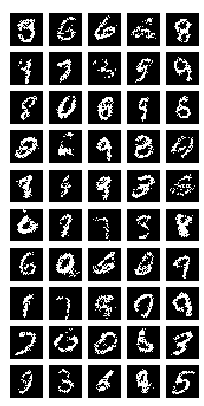
\includegraphics[height=5em]{figs/vae-sample-cropped}
										
\includegraphics[height=5em]{figs/mnist-1}
								};
								\node[right=0.3 of X2, align=center] { %label={left:$\ni$}
										
\includegraphics[height=5em]{figs/mnist-2}
								};
								\fill[opacity=0.2, structurecolor] (X.north east) -- (Z.north west) -- (Z.south west) -- (X.south east) -- cycle;
								\fill[opacity=0.2, structurecolor] (Z.north east) -- (X2.north west) -- (X2.south west) -- (Z.south east) -- cycle;
								\draw[arr] (X) to
								 	node[below,inner sep=2pt]{\small encoder}
									node[above,inner sep=2pt]{$e(Z | X)$} (Z);
								\draw[arr] (Z) to
									node[below]{\small decoder}
									node[above]{$d(X | Z)$} (X2);
							\end{tikzpicture}
							\end{center}
	            \item Objective:
	            \begin{itemize}
	                \item For each $x$, want to minimize
										% ``reconstruction error'' for each $x$ \\[-1em]
	                    % \[ \mathrm{Rec}(x) = \Ex_{z \sim e \mid x} \underbrace{~\mathrm I_{d\mid z}(x)~}_{\substack{\text{Additional bits to}\\\text{specify $x$ from $d|z$}}}
	                	%    = \sum_z e(z \mid x) \log \frac1{d(x \mid z)} \]
	                    % \[ \mathrm{Rec}(x) = - \Ex_{z \sim e \mid x} \log {d(x \mid z)} \]
	                  $\displaystyle
											\mathrm{Rec}(x) :=
												\overset{\smash{\mathclap{\text{\tiny\color{gray}``reconstruction error'' }}}}
												{ -\!\! \Ex_{z \sim e \mid x}\! \log {d(x \mid z)}} $
	                \vspace{-0.2em}
	                \item Also have a distribution $p(Z)$ that we want encodings to match.
	                    % (Uncorrelated features are more useful.)
	                \item Combine to get VaE objective:\\[0.4em] $\mathrm{ELBO}_{p,e,d}(x) :=$
										\\[-2.1em]
								  \onslide<+->{
	                	\[~~
										 -{\color{gray!80}\underbrace{\usebeamercolor[fg]{normal text} \kldiv[\big]{e(Z|x)}{p(Z)}}_{\smash{\text{\tiny divergence from prior}}}}
									   \onslide<+->{ - \mathrm{Rec}(x)}
										 \onslide<+->{= \!\!\Ex_{z \sim e|x}\! \left[\log \frac{p(z) d(x\mid z)}{e(z\mid x)}\right]}
	                    \onslide<+->{\alert<.>{\le
												\overset{{\color{gray!80}\smash{\text{\tiny ``evidence''}}}}
												{\log \Pr\nolimits_{pd}(x)}%
											}}
									 \]}
	            \end{itemize}
	        \end{itemize}
	    % \column{0.16\linewidth}
	    %     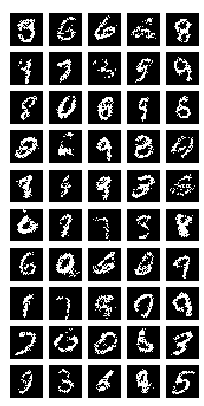
\includegraphics[width=\linewidth]{figs/vae-sample-cropped}
	    %     % 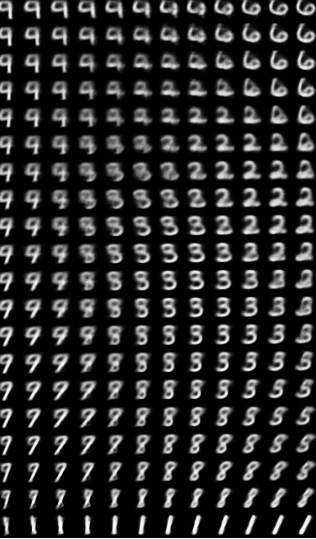
\includegraphics[width=\linewidth]{figs/vae2-cropped}
	    % \end{columns}
			\vspace{-0.7em}

	    \pause[\thebeamerpauses]
	    \alert<.(1)-.(3)>{
					Urge to use graphical models (even if can't quite capture \emph{entire} VaE)}
	    \setlength{\fboxsep}{0pt}
	    \pause\Put(-330,180){\color{structurecolor}\fbox{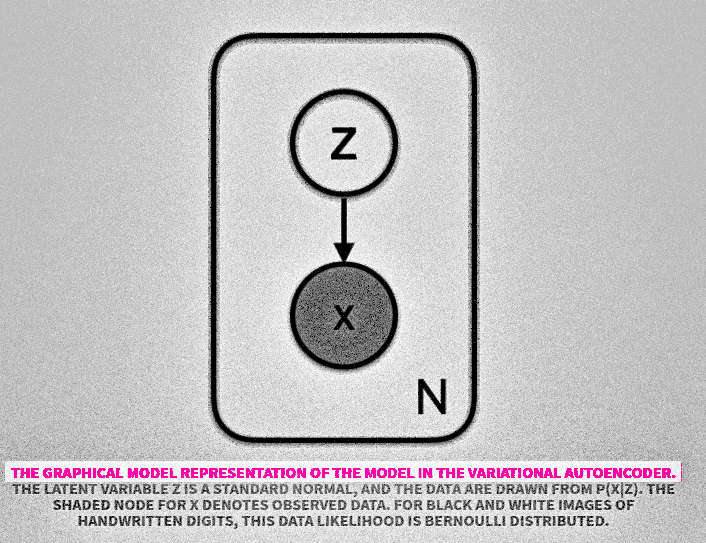
\includegraphics[height=5cm]{figs/vae-diagram-2-colored}}}
	    \pause\Put(-180,185){\color{structurecolor}\fbox{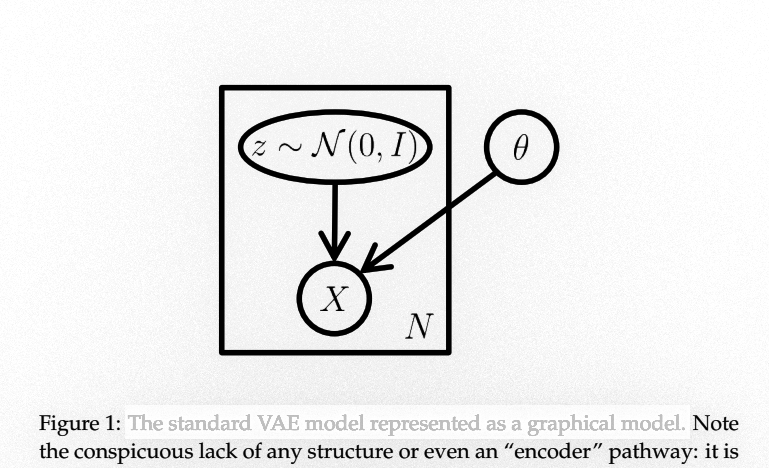
\includegraphics[height=4cm]{figs/vae-diagram-3-uncolored}}}
	    %
			\onslide<+(3)->{
				\Put(-230,195){\color{structurecolor}\fbox{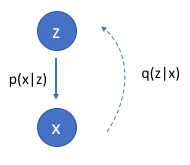
\includegraphics[height=3cm]{figs/vae-diagram-1-cropped}}}%
			}%
	    % \pause
	    % \Put(10,0){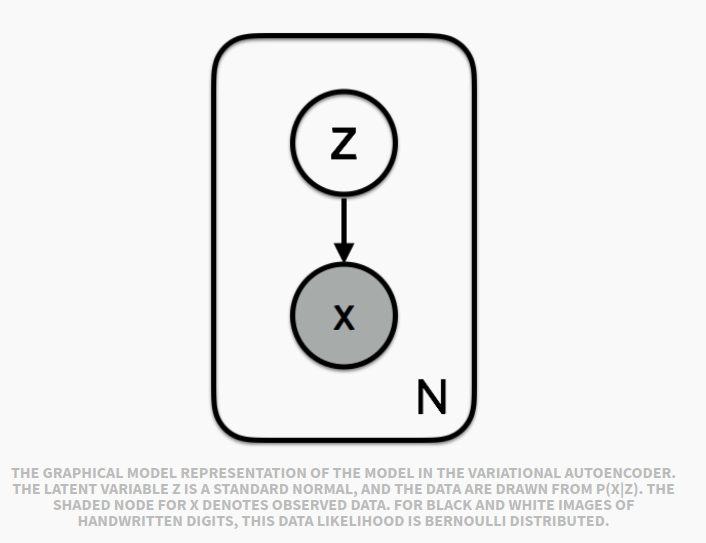
\includegraphics[height=3cm]{figs/vae-diagram-2}}
	    \begin{itemize}[<+-|alert@+>]
	        \item $e(Z\mid X)$ has same target as $p(Z)$, so can't put in BN;
	        \item The heart of the VaE is not its structure, but its objective.
	    \end{itemize}
			% \pause
		\end{frame}

	\begin{frame} \frametitle{Variational Auto-Encoders, Take 2}
			\begin{columns}[c]
			\column{0.38\textwidth}
	    \begin{itemize}[<+-|alert@+>]
	        \item Structure:
	        \begin{description}
	            % \item generate samples of $X$ from a (smaller) latent space $Z$:
	            \item[$e(Z | X)$]: encoder
							 	% encodes $X$ in a latent space $Z$;
	            \item[$d(X | Z)$]: decoder
								% generate samples of $X$ from $Z$.
	            \item[$p(Z)$]: prior
								% a prior over from $Z$.
	        \end{description}
	        \item observe a sample $x$
					% \begin{itemize}
					% 	\item and trust encoding
					% \end{itemize}
	    \end{itemize}

			\column{0.60\textwidth}
			\onslide<7->{
	    \alert<7>{Objective function is free:}}
	    \[
					\usebeamercolor{alerted text}
					\color<7>{fg}
	        \alt<7->{\aar**}{\hspace{5ex}}{
						\usebeamercolor{normal text}
						\color<7>{fg}\hspace{-1.5em}
						\begin{tikzpicture}[center base]
	            \node[dpad0] (Z) {$Z$};
	            \node[dpad0,right=.9 of Z] (X) {$X$};
	            \onslide<2->{
	                \draw[arr2, ->, onslide=<2>{alertcolor}] (X)
									 		to[bend left=60, looseness=1]
									 		% to[in=-70,out=-110, looseness=1]
											%% v1: exclamation point
	                    % node[below]{$e\onslide<5->{\alert<5>{!}}$} (Z); }
											%% v2: gray ^(\infty)
	                    % node[below, inner sep=1pt]{$e\color{gray}\onslide<6->{\alert<6>{^{\mathrlap{(\only<6>{\beta{:}}\infty)}}}}$} (Z); }
											%% v3: gray infinity, separate node.
	                    node[below]{$e$}
											node[above, inner sep=2pt]{$\lgss\onslide<6->{\alert<6>{(\only<6>{\beta{:}}\infty)}}$}
											%% v4: gray infinity above, except on first show, then with e
	                    % node[below, inner sep=2pt]{$e\only<6>{\mathrlap{\lgss\alert{(\beta{:}\infty)}}}$}
											% node[above, inner sep=2pt]{$\lgss\onslide<7->{(\infty)}$}
										(Z); }
	            \onslide<3->{
	                \draw[arr2, ->, onslide=<3>{alertcolor}] (Z)
											% to[bend left=50]
											to[bend left=60, looseness=1]
	                    node[above]{$d$} (X); }
	            \onslide<5->{
	                \draw[arr2, <<-, onslide=<5>{alertcolor}] (X) --
	                    node[above,pos=0.8]{$x$}
	                    ++(0.9, 0);}
	            \onslide<4->{
	                \draw[arr2, <-, onslide=<4>{alertcolor}] (Z) --
	                    node[above,pos=0.6]{$p$}
	                    node[below=1pt,pos=0.6]{\only<9>{$\color{alertcolor}\scriptscriptstyle(\beta?)$}}
	                    ++(-0.9, 0);}
	        \end{tikzpicture}\!\!\!}
					\onslide<7->{
						 = \mathrm{ELBO}_{p,e,d}(x) }
					% \alert<6>{\;= \mathrm{ELBO}_{p,e,d}(x)}
	    \]
			\end{columns}

			\bigskip
			\onslide<8->{
			\usebeamercolor{alerted text} \color<8>{fg}
			\[=~ \aar**{
			\usebeamercolor{normal text} \color<8>{fg}
			\begin{tikzpicture}[center base]%transform canvas={scale=1}
				\node[dpadded, outer sep=0pt, minimum height=5em] (X) at (0,0) {$X$};
				\node[dpadded, outer sep=0pt, minimum height=2.5em] (Z) at (3,0) {$Z$};
				\node[dpadded, outer sep=0pt, minimum height=5.5em] (X2) at (6,0) {$\hat X$};
				\fill[opacity=0.05, structurecolor] (X.north east) -- (Z.north west) -- (Z.south west) -- (X.south east) -- cycle;
				\fill[opacity=0.05, structurecolor] (Z.north east) -- (X2.north west) -- (X2.south west) -- (Z.south east) -- cycle;
				\draw[arr] (X) to
				 	% node[below,inner sep=2pt]{\small encoder}
				 	node[below,inner sep=2pt]{{$\scriptscriptstyle\color{gray}(\infty)$}}
					node[above,inner sep=2pt]{$e(Z | X)$} (Z);
				\draw[arr] (Z) to
					% node[below]{\small decoder}
					node[above]{$d(X | Z)$} (X2);
				%
				\draw[arr2, <<-] (X.west) -- node[above,pos=0.6]{$x$} ++(-0.6, 0);
				\draw[arr2, <<-] (X2.east) -- node[above,pos=0.6]{$x$} ++(0.6, 0);
				\draw[arr2, <-] (Z.north) -- node[left,pos=0.6]{$p$} ++(0, 0.6);
				% \draw[arr, double equals sign distance] (X) to[bend right] (X2);
			\end{tikzpicture}}
			\]}
		\end{frame}


	\begin{frame} \frametitle{Visual Proof: The Variational Bound}
			%% Visual proof: VaE Variational Bound
	    \begin{align*}
	    	\onslide<3->{- \log \Pr\nolimits_{p,d}(X\!=\!x) ~=\hspace{0.8in}&\\[-1.3em]
	    	\aar*{\begin{tikzpicture}[center base]
	    	   \node[dpad0] (Z) {$Z$};
	    	   \node[dpad0,right=.6 of Z] (X) {$X$};
	    	   \draw[arr2, ->] (Z) to[bend left=20]
	    		   node[above]{$\scriptstyle d$} (X);
	    	   \draw[arr2, <<-] (X) --
	    		   node[above,pos=0.8]{$\scriptstyle x$}
	    		   ++(0.9, 0);
	    	   \draw[arr2, <-] (Z) --
	    		   node[above,pos=0.6]{$\scriptstyle p$}
	    		   ++(-0.9, 0);%
	    	\end{tikzpicture}}}
	     	&{\onslide<4->{\color{Emerald!50!black}~\le~}}
				\onslide<2->{
		     	\aar*{\begin{tikzpicture}[center base]
		    		\node[dpad0] (Z) {$Z$};
		    		\node[dpad0,right=.6 of Z] (X) {$X$};
		    		\draw[arr2, ->] (X) to[bend left=50]
%		    			node[below]{$\scriptstyle e!$} (Z);
						node[above, inner sep=1pt]{${\lgss\Tiny\infty}$}
						node[below]{$\scriptstyle e$} (Z);
		    		\draw[arr2, ->] (Z) to[bend left=50]
		    			node[above]{$\scriptstyle d$} (X);
		    		\draw[arr2, <<-] (X) --
		    			node[above,pos=0.8]{$\scriptstyle x$}
		    			++(0.9, 0);
		    		\draw[arr2, <-] (Z) --
		    			node[above,pos=0.6]{$\scriptstyle p$}
		    			++(-0.9, 0);%
		    	\end{tikzpicture}}
	        \\[-0.7em]&\hspace{1.2in}=~ -\mathrm{ELBO}_{p,e,d}(x).}
	    \end{align*}
	   \hypertarget<3>{variational-bound}{}
			\gdef\customnav{\hyperlink{dpiframe}{\beamergotobutton{Another Visual Proof: Data Processing Inequality}}}
		\end{frame}
	\gdef\customnav{}


\begin{frame}
    \frametitle{Recap}
\end{frame}




\appendix


\section{Hyper-graphs}
	\colorlet{hypergraphcolor}{benchcolor1}
	\colorlet{simplegraphcolor}{structurecolor}
	% \setbeamercolor{background canvas}{bg=black}
	%  \setbeamercolor{normal text}{fg=white}
	%  \usebeamercolor[fg]{normal text}

	\begin{frame}[label=hypergraphextra] %%%%%         HYPER-GRAPHS AND GRAPHS      %%%%%%
		\frametitle{{\color{hypergraphcolor}Hyper-graphs?} Or merely {\color{simplegraphcolor!85}graphs}?}

		\hfill
		\begin{tikzpicture||precompiled}[center base,draw=hypergraphcolor]{grok-pre}
			\fill[fill opacity=0.07,hypergraphcolor, draw, draw opacity=0.2]
				(-0.6,0.6) rectangle (2.1, -2.1);

			\node[dpadded] (C) at (0,0) {$\mathit C$};
			\node[dpadded] (T) at (1.5,0){$\mathit T$};
			\node[dpadded] (SL) at (.75,-1.5){$\it SL$};

			\draw[arr] (T) to[bend right]  (C);
			\alert<2>{ \mergearr{C}{T}{SL} }
			% \drawbb
			\end{tikzpicture||precompiled}
		\onslide<2->{
			\hfill
			\begin{tikzpicture||precompiled}[center base]{widget}%[center base]
			\fill[fill opacity=0.07,simplegraphcolor, draw, draw opacity=0.2]
				(-2.1,-1.85) rectangle (2.1, 1.6);

				\node[dpadded] (SL) at (0,-1.3) {$\mathit{SL}$};

				\node[dpadded] (C) at (-1.5,1) {$\mathit C$};
				\node[dpadded] (T) at (1.5,1) {$\mathit T$};

				\alert<2>{
					\node[dpadded,light pad] (CT) at (0, 0){$\scriptstyle C \times T$};
					\draw[arr1, ->>] (CT) -- (C);
					\draw[arr1, ->>] (CT) -- (T);
					\draw[arr1] (CT) -- (SL);
					}
				\draw[arr] (T) to [bend right=15] (C);
				% \drawbb
				\end{tikzpicture||precompiled}
			}
			\hfill~
		\onslide<3->{
			\vspace{1em}
			\begin{itemize}
				\item<3-|alert@+> This widget expands state space, but graphs are simpler.
				\item<4-> \alert<4>{There is a natural correspondence}
				\[ \text{\color{hypergraphcolor} joint distributions}\quad\leftrightarrows\quad\parbox{15em}{\color{simplegraphcolor}\centering expanded joint distributions\\ satisfying coherence constraints} \]
			\end{itemize}
			}
		\onslide<5->
			{\small\color{gray} (working directly with hypergraphs is also possible)}

		% \vskip0pt plus 1filll
		\gdef\customnav{\hyperlink{definition}{\beamerreturnbutton{main definition}}}
		\end{frame} %----------
		\gdef\customnav{}


\section{The Information Deficiency}
	\begin{frame}[label=idefextra]\frametitle{Illustrations of $\IDef{}$}
		\def\vsize{0.4}
		\begin{center}
		% \vskip0pt plus 1filll
		% \tikzset{dpad0/.append style={fill opacity=0.1}}
		\begin{tikzpicture}[center base,scale=1.5] %\label{subfig:justXY}
			% \node[dpad0] (1) at (0,2){$\pdgunit$};
			\node[dpad0] (X) at (-0.45,.85){$X$};
			\node[dpad0] (Y) at (0.45,.85){$Y$};
			\path[fill=green!50!black] (-0.2,0) circle (\vsize) ++(-110:.26) node[label=below:\tiny$X$]{};
			\path[fill=green!50!black] (0.2,0) circle (\vsize) ++(-70:.26) node[label=below:\tiny$Y$]{};
			\begin{scope}
				\clip (-0.2,0) circle (\vsize);
				\clip (0.2,0) circle (\vsize);
				\fill[green!50!black] (-1,-1) rectangle (3,3);
				% \draw[ultra thick,white] (-0.2,0) circle (\vsize);
				% \draw[ultra thick,white] (0.2,0) circle (\vsize);
			\end{scope}
			\draw (-0.2,0) circle (\vsize);
			\draw (0.2,0) circle (\vsize);
			\useasboundingbox (current bounding box);
			\node at (-0.8, 0.4){};
			\end{tikzpicture}$\qquad$\pause
		%% EXAMPLE: X -> Y
		\begin{tikzpicture}[center base,scale=1.5]%\label{subfig:XtoY}
			% \node[dpad0] (1) at (0,2){$\pdgunit$};
			\node[dpad0] (X) at (-0.45,0.85){$X$};
			\node[dpad0] (Y) at (0.45,0.85){$Y$};
			\draw[arr] (X) to[] (Y);
			% \draw[arr] (1) to[] (Y);
			\path[fill=green!50!black] (-0.2,0) circle (\vsize) ++(-110:.26) node[label=below:\tiny$X$]{};
			\path[fill=white!70!black] (0.2,0) circle (\vsize) ++(-70:.26) node[label=below:\tiny$Y$]{};
			\begin{scope}
				\clip (-0.2,0) circle (\vsize);
				\clip (0.2,0) circle (\vsize);
				\fill[green!50!black] (-1,-1) rectangle (3,3);
				% \draw[ultra thick,white] (-0.2,0) circle (\vsize);
				% \draw[ultra thick,white] (0.2,0) circle (\vsize);
			\end{scope}
			\draw (-0.2,0) circle (\vsize);
			\draw (0.2,0) circle (\vsize);
			\useasboundingbox (current bounding box);
			\node at (-0.8, 0.4){};
			\end{tikzpicture}$\qquad$\pause
		%% EXAMPLE: X ->> Y
		\begin{tikzpicture}[center base,scale=1.5]%\label{subfig:XtoY}
			% \node[dpad0] (1) at (0,2){$\pdgunit$};
			\node[dpad0] (X) at (-0.45,0.85){$X$};
			\node[dpad0] (Y) at (0.45,0.85){$Y$};
			\draw[arr,->>] (X) to[] (Y);
			% \draw[arr] (1) to[] (Y);
			\path[fill=green!50!black] (-0.2,0) circle (\vsize) ++(-110:.26) node[label=below:\tiny$X$]{};
			\path[fill=red!50!black] (0.2,0) circle (\vsize) ++(-70:.26) node[label=below:\tiny$Y$]{};
			\begin{scope}
				\clip (-0.2,0) circle (\vsize);
				\clip (0.2,0) circle (\vsize);
				\fill[green!50!black] (-1,-1) rectangle (3,3);
				% \draw[ultra thick,white] (-0.2,0) circle (\vsize);
				% \draw[ultra thick,white] (0.2,0) circle (\vsize);
			\end{scope}
			\draw (-0.2,0) circle (\vsize);
			\draw (0.2,0) circle (\vsize);
			\useasboundingbox (current bounding box);
			\node at (-0.8, 0.4){};
			\end{tikzpicture}$\qquad$\pause
		%% EXAMPLE: X <-> Y
		\begin{tikzpicture}[center base,scale=1.5] %\label{subfig:XY-cycle}
			% \node[dpad0] (1) at (0,2){$\pdgunit$};
			\node[dpad0] (X) at (-0.45,0.85){$X$};
			\node[dpad0] (Y) at (0.45,0.85){$Y$};
			\draw[arr] (X) to[bend left] (Y);
			\draw[arr] (Y) to[bend left] (X);
			\draw[fill=white!70!black] (-0.2,0) circle (\vsize) ++(-110:.26) node[label=below:\tiny$X$]{};
			\draw[fill=white!70!black] (0.2,0) circle (\vsize) ++(-70:.26) node[label=below:\tiny$Y$]{};
			\begin{scope}
				\clip (-0.2,0) circle (\vsize);
				\clip (0.2,0) circle (\vsize);
				\fill[green!50!black] (-1,-1) rectangle (3,3);
				% \draw[ultra thick,white] (-0.2,0) circle (\vsize);
				% \draw[ultra thick,white] (0.2,0) circle (\vsize);
			\end{scope}
			\draw (-0.2,0) circle (\vsize);
			\draw (0.2,0) circle (\vsize);
			\useasboundingbox (current bounding box.south west) rectangle (current bounding box.north east);
			\node at (-0.85, 0.4){};
			\end{tikzpicture}
		\end{center}

			% \vskip0pt plus 1filll \hfill
			\gdef\customnav{%
				\hyperlink{returntosemantics}{\beamerreturnbutton{back to semantics}}}
		\end{frame}

	\begin{frame} % More IDef Illustrations
		\def\vsize{0.4}
		\def\bnslide{2}
		\def\spacerlength{0.5em}
		\begin{tikzpicture}[center base]\label{subfig:justX-0}
			\node[dpad0] (X) at (0,1){$X$};
			\draw[fill=green!50!black]  (0,0) circle (\vsize)  ++(-90:.22) node[label=below:\tiny$X$]{};
			\useasboundingbox (current bounding box);
			\node at (-0.5, 0.6){};
			\end{tikzpicture}
		\begin{tabular}{c}
				\begin{tikzpicture}[onslide=<\bnslide>{is bn}]\label{subfig:justX-1}
					\node[dpad0] (1) at (-0.4,.85){$\!\pdgunit\!$};
					\node[dpad0] (X) at (0.4,.85){$X$};
					\draw[arr1] (1)  -- (X);
					\draw[fill=white!70!black]  (0,0) circle (\vsize) ++(-90:.22) node[label=below:\tiny$X$]{};
					\node at (-0.6,0.35){};
					\useasboundingbox (current bounding box);
					\node at (-0.7, 0.35){};
					\end{tikzpicture} \\[0.5em]
				\begin{tikzpicture}\label{subfig:justX-2}
					\node[dpad0] (1) at  (-0.45,.85){$\!\pdgunit\!$};
					\node[dpad0] (X) at  (0.45,.85){$X$};
					\draw[arr1] (1) to[bend left=20] (X);
					\draw[arr1] (1) to[bend right=20] (X);
					\draw[fill=red!50!black] (0,0) circle (\vsize) ++(-90:.22) node[label=below:\tiny$X$]{};
					\useasboundingbox (current bounding box);
					\node at (-0.7, 0.35){};
					\end{tikzpicture}
			\end{tabular}%}
			\hspace{\spacerlength}\vrule\hspace{\spacerlength}
		% \adjustbox{valign=b}{
		\begin{tabular}{c}
				%% EXAMPLE: X  Y
				\begin{tikzpicture}[] \label{subfig:justXY}
					% \node[dpad0] (1) at (0,2){$\pdgunit$};
					\node[dpad0] (X) at (-0.45,.85){$X$};
					\node[dpad0] (Y) at (0.45,.85){$Y$};
					\path[fill=green!50!black] (-0.2,0) circle (\vsize) ++(-110:.23) node[label=below:\tiny$X$]{};
					\path[fill=green!50!black] (0.2,0) circle (\vsize) ++(-70:.23) node[label=below:\tiny$Y$]{};
					\begin{scope}
						\clip (-0.2,0) circle (\vsize);
						\clip (0.2,0) circle (\vsize);
						\fill[green!50!black] (-1,-1) rectangle (3,3);
						% \draw[ultra thick,white] (-0.2,0) circle (\vsize);
						% \draw[ultra thick,white] (0.2,0) circle (\vsize);
					\end{scope}
					\draw (-0.2,0) circle (\vsize);
					\draw (0.2,0) circle (\vsize);
					\useasboundingbox (current bounding box);
					\node at (-0.8, 0.4){};
					\end{tikzpicture}\\[0.5em]
				%% EXAMPLE: X -> Y
				\begin{tikzpicture}[] \label{subfig:XtoY}
					% \node[dpad0] (1) at (0,2){$\pdgunit$};
					\node[dpad0] (X) at (-0.45,0.85){$X$};
					\node[dpad0] (Y) at (0.45,0.85){$Y$};
					\draw[arr1] (X) to[] (Y);
					% \draw[arr] (1) to[] (Y);
					\path[fill=green!50!black] (-0.2,0) circle (\vsize) ++(-110:.23) node[label=below:\tiny$X$]{};
					\path[fill=white!70!black] (0.2,0) circle (\vsize) ++(-70:.23) node[label=below:\tiny$Y$]{};
					\begin{scope}
						\clip (-0.2,0) circle (\vsize);
						\clip (0.2,0) circle (\vsize);
						\fill[green!50!black] (-1,-1) rectangle (3,3);
						% \draw[ultra thick,white] (-0.2,0) circle (\vsize);
						% \draw[ultra thick,white] (0.2,0) circle (\vsize);
					\end{scope}
					\draw (-0.2,0) circle (\vsize);
					\draw (0.2,0) circle (\vsize);
					\useasboundingbox (current bounding box);
					\node at (-0.8, 0.4){};
					\end{tikzpicture}
			\end{tabular}%}
			% \hspace{\spacerlength}
		\begin{tabular}{c}
				%% EXAMPLE: X <-> Y
				\begin{tikzpicture}[center base]\label{subfig:XY-cycle}
					% \node[dpad0] (1) at (0,2){$\pdgunit$};
					\node[dpad0] (X) at (-0.45,0.85){$X$};
					\node[dpad0] (Y) at (0.45,0.85){$Y$};
					\draw[arr1] (X) to[bend left] (Y);
					\draw[arr1] (Y) to[bend left] (X);
					\draw[fill=white!70!black] (-0.2,0) circle (\vsize) ++(-110:.25) node[label=below:\tiny$X$]{};
					\draw[fill=white!70!black] (0.2,0) circle (\vsize) ++(-70:.25) node[label=below:\tiny$Y$]{};
					\begin{scope}
						\clip (-0.2,0) circle (\vsize);
						\clip (0.2,0) circle (\vsize);
						\fill[green!50!black] (-1,-1) rectangle (3,3);
						% \draw[ultra thick,white] (-0.2,0) circle (\vsize);
						% \draw[ultra thick,white] (0.2,0) circle (\vsize);
					\end{scope}
					\draw (-0.2,0) circle (\vsize);
					\draw (0.2,0) circle (\vsize);
					\useasboundingbox (current bounding box.south west) rectangle (current bounding box.north east);
					\node at (-0.85, 0.4){};
					\end{tikzpicture}\\[2.5em]
					% \hspace{\spacerlength}
				%% EXAMPLE: 1 -> Y;1->X
				\begin{tikzpicture}[center base, onslide=<\bnslide>{is bn}] \label{subfig:XYindep}
					\node[dpad0] (1) at (0,0.75){$\!\pdgunit\!$};
					\node[dpad0] (X) at (-0.7,0.95){$X$};
					\node[dpad0] (Y) at (0.7,0.95){$Y$};
					\draw[arr0] (1) to[] (X);
					\draw[arr0] (1) to[] (Y);
					\draw[fill=white!70!black] (-0.2,0) circle (\vsize) ++(-110:.23) node[label=below:\tiny$X$]{};
					\draw[fill=white!70!black] (0.2,0) circle (\vsize) ++(-70:.23) node[label=below:\tiny$Y$]{};
					\begin{scope}
						\clip (-0.2,0) circle (\vsize);
						\clip (0.2,0) circle (\vsize);
						\fill[red!50!black] (-1,-1) rectangle (3,3);
						% \draw[ultra thick,white] (-0.2,0) circle (\vsize);
					% \draw[ultra thick,white] (0.2,0) circle (\vsize);
					\end{scope}
					\draw (-0.2,0) circle (\vsize);
					\draw (0.2,0) circle (\vsize);
					\useasboundingbox (current bounding box.south west) rectangle (current bounding box.north east);
					\node at (-0.88, 0.4){};
					\end{tikzpicture}
			\end{tabular}
			\hspace{\spacerlength}
		 %% EXAMPLE: 1 -> X -> Y
		\begin{tikzpicture}[center base, onslide=<\bnslide>{is bn}]\label{subfig:1XY}
			\node[dpad0] (1) at (0.15,2){$\!\pdgunit\!$};
			\node[dpad0] (X) at (-0.45,1.4){$X$};
			\node[dpad0] (Y) at (0.35,1){$Y$};
			\draw[arr0] (1) to[] (X);
			\draw[arr1] (X) to[] (Y);
			\path[fill=white!70!black] (-0.2,0) circle (\vsize) ++(-110:.23) node[label=below:\tiny$X$]{};
			\path[fill=white!70!black] (0.2,0) circle (\vsize) ++(-70:.23) node[label=below:\tiny$Y$]{};
			\begin{scope}
				\clip (-0.2,0) circle (\vsize);
				\clip (0.2,0) circle (\vsize);
				% \fill[red!50!black] (-1,-1) rectangle (3,3);
				% \draw[ultra thick,white] (-0.2,0) circle (\vsize);
				% \draw[ultra thick,white] (0.2,0) circle (\vsize);					\end{scope}
			\end{scope}
			\draw (-0.2,0) circle (\vsize);
			\draw (0.2,0) circle (\vsize);
			\useasboundingbox (current bounding box);
			\node at (-0.7, 0.6){};
			\end{tikzpicture}
			% \hspace{\spacerlength}\hspace{2.5pt}\vrule\hspace{2.5pt}\hspace{\spacerlength}
		\relax	%CENTER CODE.
			\vspace{0.5em}
			\onslide<bnslide>{\tikz[is bn] \node{Achievable by BN}; }

		%% EXAMPLE: 1 -> X -> Y -> Z
		\begin{tikzpicture}[center base, onslide=<\bnslide>{is bn}] \label{subfig:1XYZ}
			% \node[dpad0] (1) at (-0.5,2.3){$\!\pdgunit\!$};
			% \node[dpad0] (X) at (-0.5,1.5){$X$};
			% \node[dpad0] (Y) at (0.35,1.25){$Y$};
			% \node[dpad0] (Z) at (0.25,2.25){$Z$};
			\node[dpad0] (1) at (-1,0.8){$\!\pdgunit\!$};
			\node[dpad0] (X) at (-0.6,1.6){$X$};
			\node[dpad0] (Y) at (0.35,1.6){$Y$};
			\node[dpad0] (Z) at (1.0,0.9){$Z$};
			\draw[arr0] (1) to (X);
			\draw[arr1] (X) to[] (Y);
			\draw[arr1] (Y) to[] (Z);
			\path[fill=white!70!black] (210:0.22) circle (\vsize) ++(-130:.25) node[label=below:\tiny$X$]{};
			\path[fill=white!70!black] (-30:0.22) circle (\vsize) ++(-50:.25) node[label=below:\tiny$Y$]{};
			\path[fill=white!70!black] (90:0.22) circle (\vsize) ++(40:.29) node[label=above:\tiny$Z$]{};
			\begin{scope}
				\clip (90:0.22) circle (\vsize);
				\clip (210:0.22) circle (\vsize);
				\fill[red!50!black] (-1,-1) rectangle (3,3);
				% \draw[ultra thick,white] (210:0.2) circle (\vsize);
				% \draw[ultra thick,white] (90:0.2) circle (\vsize);
				\clip (-30:0.22) circle (\vsize);
				\fill[white!70!black] (-1,-1) rectangle (3,3);
				% \draw[ultra thick,white] (-30:0.2) circle (\vsize);
				% \draw[ultra thick,white] (210:0.2) circle (\vsize);
				% \draw[ultra thick,white] (90:0.2) circle (\vsize);
			\end{scope}
			\begin{scope}
				\draw[] (-30:0.22) circle (\vsize);
				\draw[] (210:0.22) circle (\vsize);
				\draw[] (90:0.22) circle (\vsize);
			\end{scope}
			\useasboundingbox (current bounding box);
			\node at (-0.7, 0.7){};
			\end{tikzpicture}
			\hspace{\spacerlength}
		%% EXAMPLE: X -> Y -> Z -> X
		\begin{tikzpicture}[center base] \label{subfig:XYZ-cycle}
			% \node[dpad0] (1) at (-0.5,2.3){$\pdgunit$};
			\node[dpad0] (X) at (-0.5,1.75){$X$};
			\node[dpad0] (Y) at (0.35,1.25){$Y$};
			\node[dpad0] (Z) at (0.25,2.25){$Z$};
			% \draw[arr0] (1) to (X);
			\draw[arr1] (X) to[bend right=25] (Y);
			\draw[arr1] (Y) to[bend right=25] (Z);
			\draw[arr1] (Z) to[bend right=25] (X);
			%option: -- either X -> Y -> Z -> X, or <-> Y <-> Z <-> X. For the latter, uncomment the 6 lines below and comment out the next 3.
			% \draw[arr1] (Z) to[bend left=5] (Y);
			% \draw[arr1] (Y) to[bend left=5] (X);
			% \draw[arr1] (X) to[bend left=5] (Z);
			% \draw[fill=red!50!black] (210:0.22) circle (\vsize) ++(-130:.27) node[label=below:\tiny$X$]{};
			% \draw[fill=red!50!black] (-30:0.22) circle (\vsize) ++(-50:.27) node[label=below:\tiny$Y$]{};
			% \draw[fill=red!50!black] (90:0.22) circle (\vsize) ++(140:.31) node[label=above:\tiny$Z$]{};

			% grey filling for one covering.
			\draw[fill=white!70!black] (210:0.22) circle (\vsize) ++(-130:.27) node[label=below:\tiny$X$]{};
			\draw[fill=white!70!black] (-30:0.22) circle (\vsize) ++(-50:.27) node[label=below:\tiny$Y$]{};
			\draw[fill=white!70!black] (90:0.22) circle (\vsize) ++(40:.31) node[label=above:\tiny$Z$]{};

			\begin{scope}
				\clip (-30:0.22) circle (\vsize);
				\clip (210:0.22) circle (\vsize);
				% \fill[white!70!black] (-1,-1) rectangle (3,3);
				\clip (90:0.22) circle (\vsize);
				\fill[green!50!black] (-1,-1) rectangle (3,3);
			\end{scope}
			\begin{scope}
				\draw[] (-30:0.22) circle (\vsize);
				\draw[] (210:0.22) circle (\vsize);
				\draw[] (90:0.22) circle (\vsize);
			\end{scope}
			\useasboundingbox (current bounding box);
			\node at (-0.7, 0.7){};
			\end{tikzpicture}
			\hspace{\spacerlength}
		%% EXAMPLE: X -> Y <- Z
		\begin{tikzpicture}[center base] \label{subfig:XZtoY}
			% \node[dpad0] (1) at (-0.5,2.3){$\pdgunit$};
			\node[dpad0] (X) at (-0.45,1.9){$X$};
			\node[dpad0] (Y) at (0.3,1.25){$Y$};
			\node[dpad0] (Z) at (0.4,2.15){$Z$};
			% \draw[arr0] (1) to (X);
			\draw[arr0] (X) to[] (Y);
			\draw[arr1] (Z) to[] (Y);
			\path[fill=green!50!black] (210:0.22) circle (\vsize) ++(-130:.25) node[label=below:\tiny$X$]{};
			\path[fill=red!50!black] (-30:0.22) circle (\vsize) ++(-50:.25) node[label=below:\tiny$Y$]{};
			\path[fill=green!50!black] (90:0.22) circle (\vsize) ++(40:.29) node[label=above:\tiny$Z$]{};
			\begin{scope}
				\clip (-30:0.22) circle (\vsize);
				\clip (90:0.22) circle (\vsize);
				\fill[white!70!black] (-1,-1) rectangle (3,3);
			\end{scope}
			\begin{scope}
				\clip (-30:0.22) circle (\vsize);
				\clip (210:0.22) circle (\vsize);
				\fill[white!70!black] (-1,-1) rectangle (3,3);

				\clip (90:0.22) circle (\vsize);
				\fill[green!50!black] (-1,-1) rectangle (3,3);
				% \draw[ultra thick,white] (210:0.2) circle (\vsize);
				% \draw[ultra thick,white] (90:0.2) circle (\vsize);
				% \draw[ultra thick,white] (-30:0.2) circle (\vsize);
				% \draw[ultra thick,white] (210:0.2) circle (\vsize);
				% \draw[ultra thick,white] (90:0.2) circle (\vsize);
			\end{scope}
			\draw[] (-30:0.22) circle (\vsize);
			\draw[] (210:0.22) circle (\vsize);
			\draw[] (90:0.22) circle (\vsize);
			\useasboundingbox (current bounding box);
			% \node at (-0.7, 0.7){};
			\end{tikzpicture}
			\hspace{\spacerlength}
		%% EXAMPLE: X <-> Y <-> Z
		\begin{tikzpicture}[center base] \label{subfig:XYZ-bichain}
			% \node[dpad0] (1) at (0.1,2.4){$\pdgunit$};
			\node[dpad0] (X) at (-1,1.2){$X$};
			\node[dpad0] (Y) at (0,1.7){$Y$};
			\node[dpad0] (Z) at (1,1.4){$Z$};
			% \draw[arr1] (1) to (X);
			% \draw[arr1] (1) to (Y);
			\draw[arr1] (X) to[bend right=15] (Y);
			\draw[arr1] (Y) to[bend right=15] (X);
			\draw[arr1] (Y) to[bend right=15] (Z);
			\draw[arr1] (Z) to[bend right=15] (Y);
			\path[fill=white!70!black] (210:0.22) circle (\vsize) ++(-130:.25) node[label=below:\tiny$X$]{};
			\path[fill=red!50!black] (-30:0.22) circle (\vsize) ++(-50:.25) node[label=below:\tiny$Y$]{};
			\path[fill=white!70!black] (90:0.22) circle (\vsize) ++(40:.29) node[label=above:\tiny$Z$]{};
			\begin{scope}
				\clip (-30:0.22) circle (\vsize);
				\clip (90:0.22) circle (\vsize);
				\fill[white!70!black] (-1,-1) rectangle (3,3);
			\end{scope}
			\begin{scope}
				\clip (90:0.22) circle (\vsize);
				\clip (210:0.22) circle (\vsize);
				\fill[red!50!black] (-1,-1) rectangle (3,3);
			\end{scope}
			\begin{scope}
				\clip (-30:0.22) circle (\vsize);
				\clip (210:0.22) circle (\vsize);
				\fill[white!70!black] (-1,-1) rectangle (3,3);

				\clip (90:0.22) circle (\vsize);
				\fill[green!50!black] (-1,-1) rectangle (3,3);
				% \draw[ultra thick,white] (210:0.2) circle (\vsize);
				% \draw[ultra thick,white] (90:0.2) circle (\vsize);
				% \draw[ultra thick,white] (-30:0.2) circle (\vsize);
				% \draw[ultra thick,white] (210:0.2) circle (\vsize);
				% \draw[ultra thick,white] (90:0.2) circle (\vsize);
			\end{scope}
			\draw[] (-30:0.22) circle (\vsize);
			\draw[] (210:0.22) circle (\vsize);
			\draw[] (90:0.22) circle (\vsize);
			\useasboundingbox (current bounding box);
			\node at (-0.7, 0.7){};
			\end{tikzpicture}
		\end{frame}
		\gdef\customnav{}

\section{More on Semantics}
	\begin{frame}[label=more-semantics-properties]
		\begin{prop}[{{\itshape\normalfont {uniqueness for small $\gamma$}}}]
			\begin{enumerate}
			\item If  $0 < \gamma \leq \min_L \beta_L^{\dg M}$, then
			$\bbr{\dg M}_\gamma^*$ is a singleton.
			\item $\displaystyle\lim_{\gamma\to0}\bbr{\dg M}_\gamma^*$ exists and is a singleton.
			\end{enumerate}
		\end{prop}
		\pause
		This lets us define~ $\bbr{\dg M}^* := $
		unique element $\displaystyle\left(\lim_{\gamma\to0} \bbr{\dg M}_\gamma^*\right)$.
		\end{frame}
	\begin{frame}[label=semantics-relationships]
		\frametitle{Relationships Between Semantics}
		\begin{prop}%
				% [{\normalsize{\it $\SD{\dg M}$ is the zero set of $\bbr{\dg M}$\;}}]
				[{\small{\it the set of consistent distributions is the zero set of the scoring function}}]
			$\SD{\dg M} \!= \big\{ \mu : \bbr{\dg M}_0(\mu) \!=\! 0 \big\}$.
			\end{prop}

		\begin{prop}[{\normalsize{\it If there there are distributions consistent
			 		with $\dg M$, the best distribution is one of them.\;}}]
					\label{prop:consist}
				$\bbr{\dg M}^* \in \bbr{\dg M}_0^*$, so if $\dg M$ is consistent,
				then $\bbr{\dg M}^* \in \SD{\dg  M}$.
			\end{prop}

		\gdef\customnav{\hyperlink{semantics-properties}{\beamerreturnbutton{back to semantics properties}}}
		\end{frame}
		\gdef\customnav{}


	\begin{frame}[label=another-semantics]\frametitle{Another View of PDG semantics}
		\[ \bbr{\dg M}_\gamma(\mu) = \Ex_{\mu}\log \prod_{\ed LXY} \left(\frac{\mu(Y\mid X)}{\bp(Y\mid X)}\right)^{\beta\ssub L}
		\;
		\left(\frac{\mu(\N)}{\prod\limits_{\ed LXY} \mu(Y\mid X)^{\alpha\ssub L}}\right)^\gamma
		\]
	\end{frame}

	\begin{frame}[label=another-semantics+fg] %%%%%  SCORING FUNCTION BREAKDOWN  %%%%
		% \begin{prop}\label{prop:nice-score}%
			% Let $x^{\mat w}$, $y^{\mat w}$ denote the values of
			% $X$,$Y$ in world $\mat w$. Then:
			\frametitle{Comparing PDG to Factor Graph Semantics}

			{\small
			\begin{equation*}\label{eq:semantics-breakdown}
				% \begin{split}
					\bbr{\dg M}(\mu) =
					% \Ex_{\mat w \sim \mu}\! \Bigg\{
					\Ex\nolimits_\mu	\!\!
					 \sum_{ X \xrightarrow{\!\!L} Y  }
					\bigg[\,
					    {\color{benchcolor1}\overbrace{\color{black}
					      % \beta_L \log \frac{1}{\bp(y^{\mat w} |x^{\mat w})}
					      \beta\ssub L \log \frac{1}{\bp(Y|X)}
						}^{\color{benchcolor1}\smash{\mathclap{\text{log likelihood / cross entropy}}}}}~+
						 % \qquad\qquad\qquad\\[-0.7em]\qquad\qquad
					    {\color{benchcolor2}\underbrace{\color{black}
					({\alpha \ssub L}\gamma - \beta\ssub L )
							% \log \frac{1}{\mu(y^{\mat w} |x^{\mat w})}
							\log \frac{1}{\mu(Y | X)}
						}_{\color{benchcolor2}\smash{\mathclap{\text{local regularization (if $\beta\ssub L >	\alpha\ssub L
						\gamma$)}}}}}~\bigg] - \color{structurecolor!70!blue}
						\overbrace{\color{black}
					% \gamma \log \frac{1}{\mu(\mat w)}
					\gamma \H(\mu) \vphantom{\Big|}
						}^{\color{structurecolor!70!blue}\smash{\mathclap{\text{%
							% ~~~~global regularization
							global regularization~~~~%
							}}}}\color{black}
									% \Bigg\} .				\end{split}
									.
				\end{equation*}}
			\bigskip

			\pause
			And the weighted factor graph's canonical scoring function:
			\[ \VFE_\Psi(\mu) := \Ex_{\mu} \left[ \sum_{J \in \mathcal J} {\theta_J} \log \frac1{\phi_J(X_J)} \right] - \H(\mu) \]
			% \end{prop}
		\end{frame}

	\begin{frame}[label=minimization-semantics-properties] \frametitle{Properties of Inconsistency, for minimization}

			\[ \aar{\dg M}_\gamma := \inf_\mu \bbr{\dg M}_\gamma \]
			% \begin{prop}

			Nice properties for minimization:
			\begin{itemize}
				\item The function $\gamma\mapsto\aar{\dg M}_\gamma$ is continuous for all $\gamma$
				\item The function $p \mapsto \aar{\dg M \sqcup p}_\gamma$ is smooth and strictly convex on its interior.
			\end{itemize}
				% \end{prop}
		\end{frame}

	\begin{frame}[label=semantics-thermo]
		\[ \VFE_\Phi(\mu) := \Ex_{\mu} \Big[ - \sum_{J \in \mathcal J}
			% \only<7->{\alert<7>{\theta_J}}
			\theta_J
			 \log {\phi_J(X_J)} \Big] - \H(\mu) \]
		\gdef\customnav{\hyperlink{factor-graph-intro}{\beamerreturnbutton{Back to Factor Graph Definition}}}
		\end{frame}
		\gdef\customnav{}

	\begin{frame} \frametitle{Full Factor Graph Results}
		\begin{theorem}[PDGs are WFGs]\label{thm:pdg-is-wfg}
			If $\boldsymbol\beta = \gamma\boldsymbol\alpha $, then
			$\bbr{\dg M}^*_\gamma = \Pr_{(\Phi_{\dg M}, \boldsymbol\beta)}$.


			Concretely, for all unweighted PDGs $\dg{N}$ and non-negative vectors $\mat v$
			over the edges of $\dg N$, and all $\gamma > 0$, we have that
			$\bbr{(\dg N, \mat v, \gamma \mat v)}_{\gamma}
			= \gamma\,\VFE_{(\Phi_{\dg N}, \mat v)} $; consequently,
			$\bbr{(\dg N,  \mat v,  \gamma\mat v)}_{\gamma}^*
					= \{\Pr_{(\Phi_{\dg N}, \mat v)} \}$.
		\end{theorem}

		\begin{theorem}[WFGs are PDGs]\label{them:wfg-is-pdg}
			For all weighted factor graphs $\Psi = (\Phi,\theta)$ and all $\gamma > 0$,
			we have that
			$\VFE_\Psi
			= \nicefrac1{\gamma} \bbr{{\dg M}_{\Psi,\gamma}}_{\gamma}
			+ C$
			for some constant $C$, so
			$\Pr_{\Psi}$ is the unique element of
			$\bbr{{\dg M}_{\Psi,\gamma}}_{\gamma}^*$.
			\end{theorem}

		\gdef\customnav{%
			\hyperlink{returnto-pdg-is-wfg}{\beamerreturnbutton{PDG$\to$WFG}}
			\hyperlink{returnto-pdg-is-wfg}{\beamerreturnbutton{WFG$\to$PDG}}
		}%
		\end{frame}
		\gdef\customnav{}


\section{More Losses}
\begin{frame} %% Marginal Surprise as Inconsistency
    \frametitle{Variations: Surprise as Inconsistency}
    % For partial observations
    \begin{prop}[marginal information as inconsistency]<+-|alert@+>
        If $p(X,Z)$ is a joint distribution, the (marginal) information of the (partial) observation $X=x$ is given by\\[-1.0em]
    % Marginal Information:
        \[
    	 	\I_p(x) = \log \frac{1}{p(x)} =
    		 \aar[\Bigg]{
    			\begin{tikzpicture}[center base]
    				\node[dpad0] (Z) {$Z$};
    				\node[dpad0,right=.5 of Z] (X) {$X$};
    				\coordinate (A) at ($ (X)!.5!(Z) + (0,0.7)$);
    				\draw[arr1] (A) -- node[right]{$\scriptstyle p$} ++(0,-0.25) -- (X);
    				\draw[arr1] (A) -- ++(0,-0.25) -- (Z);
                	%
    				\draw[arr2, <<-] (X) --  node[above,pos=0.8]{$\scriptstyle x$} ++(0.9, 0);
    			\end{tikzpicture}
    			}.
        \]
    \end{prop}

    % And for an entire dataset at once:
    % \begin{prop}[cross entropy as inconsistency]<+-|alert@+>
    %     Given a dataset $\xsamp$,
    %     the cross entropy $\mathrm{CE}(p,\xsamp) := -\frac{1}{|\xsamp|}\sum_{x \in \xsamp} \log p(x)$ is the inconsistency of the PDG containing $p$ and the data distribution $\datadist\xsamp$, plus the entropy of the data distribution (constant in $p$). That is,
    % 	\[
    % 	\mathrm{CE}(p;\xsamp) =
    % 	 \aar[\Bigg]{
    % 	 % \Inc\left(
    % 		\begin{tikzpicture}[center base]
    % 			\node[dpad0] (Z) {$Z$};
    % 			\node[dpad0,right=.5 of Z] (X) {$X$};
    % 			\coordinate (A) at ($ (X)!.5!(Z) + (0,0.7)$);
    % 			\draw[arr1] (A) -- node[right]{$p$} ++(0,-0.25) -- (X);
    % 			\draw[arr1] (A) -- ++(0,-0.25) -- (Z);
    % 			%
    % 			\draw[arr1, <-] (X) --  node[above,pos=0.8]{$\datadist\xsamp!$} ++(0.9, 0);
    % 			% \draw[arr1, <-] (Z) -- node[above]{$\scriptstyle q$} ++(-0.9, 0);
    % 		\end{tikzpicture}
    % 		}%_{\!\!0}
    % 		% \right)
    % 		+ \H(\datadist\xsamp).
    % 	\]
    % \end{prop}

	\begin{prop}[{\small supervised setting: conditional cross entropy}]<+->
		% Consider a cpd $f(Y \mid X)$.
		The inconsistency of the PDG containing $f(Y\mid X)$ and a high-confidence empirical distribution $\datadist\xysamp$ of samples $\xysamp = \{(x_i,y_i)\}$ is equal to the cross entropy {\color{gray}\small( plus $\H(Y\mid X)$, a constant that depends only on the data $\datadist\xysamp$)}. That is,\\[-1.4em]
		\[ \aar**{
			\begin{tikzpicture}[center base]
				\node[dpad0] (Y) {$Y$};
				\node[dpad0,left=.9 of Y] (X) {$X$};
				\coordinate (A) at ($ (X)!.5!(Y) + (0,0.8)$);
				\draw[arr1] (A) --
					node[left]{$\datadist\xysamp$}
					node[right]{$\scriptscriptstyle\color{gray!80}(\beta:\infty)$}
					++(0,-0.25) -- (X);
				\draw[arr1] (A) -- ++(0,-0.25) -- (Y);
				\draw[arr2, ->] (X) --  node[below,pos=0.5]{$f$} (Y);
			\end{tikzpicture}} = \frac1{|\xysamp|}\sum_{(x,y) \in \xysamp} \left[ \log \frac1{f(y \mid x)}\right] \quad - \H_{\datadist\xysamp}(Y\mid X).
		\]
	\end{prop}
\end{frame}


\begin{frame}[label=accuracyframe]%% Acuracy as Inconsistency
    \begin{prop}[Accuracy as Inconsistency]
        % If $h: X \to Y$ is a predictor for an input space $X$ and label space $Y$, and $f: X \to Y$ generates the correct labels, then the inconsistency of believing $f$ and $h$ (with any degree of confidence), and also that inputs are distributed according to $D(X)$, equals the information content of learning that $f(X) = h(X)$ according to $D$ (which is the log accuracy of the predictor $h$) times the confidence in $D$. That is,
        Consider a predictor $h : X \to Y$ for true labels $f : X \to Y$, and a distribution $D(X)$. The inconsistency of believing all three is
	\begin{equation*}%\label{eq:accuracy-pdg}
		\aar*{\begin{tikzpicture}[center base]
				\node[dpad0] (Y) {$Y$};
				\node[dpad0,left=1.1 of Y] (X) {$X$};
				%
				\draw[arr2, ->>] (X) to[bend left] node[pos=0.5, above]{$h$} (Y);
				\draw[arr2, ->>] (X) to[bend right] node[pos=0.5, below]{$f$} (Y);
				\draw[arr2, <-] (X) to
					node[pos=0.6, anchor=south west, above]
					% {$\overset{(\beta)}D$}
					%{$D^{\color{gray}(\beta)}$}
					{$D$}
					node[below=1pt,pos=0.6]{{$\color{gray}\scriptscriptstyle(\beta)$}}
				 +(-1.1, 0);
			\end{tikzpicture}}
		=  - \beta\,\log \Big( \mathrm{accuracy}_{f,D} (h) \Big)
		= \beta\, \I_D [f = h].
	\end{equation*}
    \end{prop}
		\pause
		\begin{itemize}[<+->]
			\item Thought of as a feature of $h$, but as a PDG, symmetry between $f,h$ is clear.
		\end{itemize}
	\end{frame}
	%
	%
	\begin{frame}[label=MSEframe] %% MSE as Inconsistency
    \begin{prop}[Mean Square Error as Inconsistency]<+->
        \begin{align*}
		\aar**{\begin{tikzpicture}[center base]
			\node[dpad0] (Y) {$Y$};
			\node[dpad0,left=1.1 of Y] (X) {$X$};
			%
			\draw[arr2, ->] (X) to[bend left]
				node[pos=0.5, above] {$\mathcal N(f(x), 1)$} (Y);
			\draw[arr2, ->] (X) to[bend right] node[pos=0.5, below]{$\mathcal N(g(x), 1)$} (Y);
			\draw[arr2, <-] (X) to
				node[pos=0.6, above]{$D$}
				node[below=1pt,pos=0.6]{{$\color{gray}\scriptscriptstyle(\beta:\infty)$}}
				 +(-1.1, 0);
		\end{tikzpicture}}
    %		&=
    %		\aar**{\begin{tikzpicture}[center base]
    %			\node[dpad0] (Y) {$Y$};
    %			\node[dpad0,left=2.2 of Y] (X) {$X$};
    %			\node[dpad0,above right=0.1 and 0.8 of X] (mf) {$\mu_f$};
    %			\node[dpad0,below right=0.1 and 0.8 of X] (mh) {$\mu_h$};
    %			%
    %			\draw[arr2, ->>] (X) to[bend left=0]
    %				node[pos=0.5, above left=0] {$f$} (mf);
    %			\draw[arr2, ->>] (X) to[bend right=0]
    %				node[pos=0.5, below left=0] {$h$} (mh);
    %			%
    %			\draw[arr2, <-] (X) to node[pos=0.6, above]{$D!$} +(-1.1, 0);
    %			%
    %			\draw[arr2, ->] (mh) to[bend right=0]
    %				node[pos=0.3, below right=0] {$\mathcal N_1$} (Y);
    %			\draw[arr2, ->] (mf) to[bend left=0]
    %				node[pos=0.3, above right=0]{$\mathcal N_1$} (Y);
    %			% \draw[arr2, <-] (X) to node[pos=0.6, above]{$D$} +(-1.1, 0);
    %		\end{tikzpicture}}\\
    		 &= \Ex\nolimits_D \Big( f(X) - h(X) \Big)^2
    		 =: \mathrm{MSE}( f, h )
	\end{align*}
    %	where $\mathcal N_1 = \mathcal N(-,1)$ is the normal distribution with unit variance, and mean equal to its argument.
    \end{prop}
\end{frame}

\subsection{Regularizers}
\begin{frame}[label=regularizationframe] %% Regularization
    \setbeamercolor{block body}{bg=gray!10!white}
	\setbeamercolor{block title}{bg=gray!45!white}
    \colorlet{priorcolor}{red}
    \begin{prop}[Regularizers as priors]
        \onslide<1->{%
            Suppose you believe $Y \sim f_\theta(Y)$,
        }\onslide<2->{%
            have a prior {\color{priorcolor}$p(\theta)$},
        }\onslide<3->{\alert<3>{%
            % and have an empirical distribution $D(Y)$ which you trust.
            and an empirical distribution $D(Y)$ which you trust.
        }}\onslide<4->{\alert<4>{%
            Then the inconsistency of also believing $\Theta = \theta_0$ is
        }}\onslide<5->{\alert<5>{%
            the {\color{priorcolor}\emph{regularized}}-cross entropy loss, and controlled by the strength $\beta_p$ of the prior.} That is,
        }
        \only<-4>{\par\vspace{-1.1em}That is,}
    	\begin{equation*}%\label{eq:regularize}
    		\aar**{\!\!\begin{tikzpicture}[center base]
    			\node[dpad0] (theta) {$\Theta$};
    			\node[dpad0, right=0.8 of theta] (Y) {$Y$};
    			%
    			\draw[arr] (theta) --
    	 			% node[above]{$\overset{{\color{gray}(\beta_f)}}f$}
    	 			% node[above]{$f^{{\color{gray}(\beta_f)}}$}
    	 			node[above]{$f$}
    				(Y);
                \onslide<2->{
        			\draw[arr, <-, priorcolor] (theta) --
        				node[above right=-2pt and -2pt, pos=0.7] {$p$}
        				node[below left=-3pt and -4pt,pos=0.6]{{$\color{red!20!gray}\scriptscriptstyle(\beta)$}}
        				++(-1.0, 0.5);}

                \onslide<4->{
                    \draw[arr, <<-, onslide=<4>{alertcolor}] (theta) --
                        node[below,pos=0.4]{$\theta_0$} ++(-1.1, -0.3);}
                \onslide<3->{
                    \draw[arr, <-, onslide=<3>{alertcolor}] (Y) --
                    	node[above,pos=0.6]{$D$}
                    	node[below=-1pt,pos=0.6]{{$\color{gray}\scriptscriptstyle(\infty)$}}
                    	 ++(1.1, 0); }
    		\end{tikzpicture}\!\!}
    		\onslide<4->{=\!}\onslide<5->{\alert<5>{
        		% \beta_f\,
        		\Ex_{y \sim D} \left[\log \frac{1}{f(y \mid \theta_0)} \right]
        			\!+ {\color{priorcolor}\beta \log \frac1{p(\theta_0)}}
        		 - \H(D)}}
    	\end{equation*}
    \end{prop}

    \onslide<7->{
        Using a (discretized) unit gaussian as a prior, $p(\theta) = \frac{1}{k} \exp(-\frac12 \theta^2)$ for a normaization constant $k$, the RHS %of \eqref{eq:regularize}
        becomes
        \[ \underbrace{\Ex\nolimits_{D} \left[\log \frac{1}{f(Y \mid \theta_0)} \right]}
        	_{\substack{\text{Cross entropy loss of $f_\theta$ w.r.t. $D$}\\(\text{data-fit cost of $\theta_0$})}}%(f_\theta; D)
        	+{\color{priorcolor} \underbrace{~\frac\beta2 \theta_0^2~}_{\substack{\ell_2 \text{ regularizer}\\(\text{complexity cost of $\theta_0$})}}} \quad
        	{\color{gray!50} \underbrace{+  \beta \log k - \H(D)}_{\text{constant in $f$ and $\theta_0$}}}. \]
        }
    % which is the $\ell_2$ regularized version of \cref{prop:many-equal-simple}.
    % Moreover, the regularization strength corresponds exactly to the confidence $\beta$ functions as the hyperparameter, a feature unique to our approach.
	\gdef\customnav{\hyperlink{bigtableframe}{\beamerreturnbutton{back to table of losses}}}
\end{frame}

\gdef\customnav{}

\section{More Visual Proofs}
\begin{frame}[t,label=dpiframe] \frametitle{Visual Proof: Data Processing Inequality}
		%% Visual Proof: DPI
		%
		\tikzset{ci2/.style={inner sep=2pt, align=center}}%
		%
		\colorlet{pcolor}{Plum}%
		\colorlet{qcolor}{MidnightBlue}%
		\def\amt{45}%
		\tikzset{pstyle/.style={line width=0.9pt, pcolor!\amt!black}}%
		\tikzset{qstyle/.style={line width=1.3pt, qcolor!\amt!black}}%
		\tikzset{pqstyle/.style={line width=1.5pt,pcolor!50!qcolor!\amt!black}}%
		%
		\def\plabel{{$\lgss\color{pcolor!40}({\beta})$}}
		\def\qlabel{{$\lgss\color{qcolor!40}({\zeta})$}}
		\def\pdgdiv{\thickD^{\mathrm{P\mskip-2muD\mskip-1.5muG}}_{\lgss({\color{pcolor!40}\beta},{\color{qcolor!40}\zeta})}\infdivx[\Big]}
		%
		{\color{structurecolor}
			\[ \pdgdiv pq \ge \pdgdiv {f\circ p}{f \circ q}\]}%
		%
    \begin{align*}%
    	% - \log \Pr\nolimits_{p,d}(X\!=\!x) ~=\qquad&\\
    	\aar*{\begin{tikzpicture}[center base]
    	   \node[dpad0] (X) {$X$};
    	   \draw[arr2, <-,qstyle] (X) --
	  		  node[above,pos=0.6,ci2]{$\scriptstyle q$}
					 % node[above,pos=0.6]{$q^{{\color{gray}(s)}}$}
					node[below, pos=0.65,ci2] {\qlabel}
    		   ++(1.1, 0);
    	   \draw[arr2, <-,pstyle] (X) --
				 	node[above,pos=0.6,ci2]{$\scriptstyle p$}
    		   % node[above,pos=0.6]{$p^{{\color{gray}(r)}}$}
					node[below, pos=0.65, ci2] {\plabel}
    		   ++(-1.1, 0);%
    	\end{tikzpicture}}
        &\onslide<2->{=
        \aar**{\begin{tikzpicture}[center base]
           \node[dpad0] (X) {$X$};
           \node[dpad0,above=.8 of X,align=center] (Y) {$Y$};
           \draw[arr2, <-,qstyle] (X) --
	            node[above,pos=0.6,ci2]{$\scriptstyle q$}
							node[below, pos=0.65,ci2] {\qlabel}
               ++(1.1, 0);
           \draw[arr2, <-,pstyle] (X) --
              node[above,pos=0.6,ci2]{$\scriptstyle p$}
							node[below, pos=0.65,ci2] {\plabel}
               ++(-1.1, 0);%
           \draw[arr2, pqstyle] (X) --
              node[left,pos=0.45,ci2]{$\scriptstyle f$}
							node[right, pos=0.45, inner sep=1pt, align=center] % below,rotate=90
							 	{{$\lgss\color{pcolor!50!qcolor!40}(\beta+\zeta)$}}
              (Y);%
        \end{tikzpicture}}} \\
        &\onslide<3->{=
        \aar**{\begin{tikzpicture}[center base]
           \node[dpad0] (X1) {$X_1$};
           \node[dpad0, right=0.7 of X1] (X2) {$X_2$};
           \node[dpad0,above=.8 of {$(X1)!.5!(X2)$},align=center] (Y) {$Y$};
           \draw[arr2, -, double equal sign distance] (X1) to (X2);
           \draw[arr2, <-,qstyle] (X2) --
              node[above,pos=0.6,ci2]{$\scriptstyle q$}
							node[below, pos=0.65,ci2] {\qlabel}
              ++(1.1, 0);
           \draw[arr2, <-,pstyle] (X1) --
              node[above,pos=0.6,ci2]{$\scriptstyle p$}
							node[below, pos=0.65,ci2] {\plabel}
              ++(-1.1, 0);%
           \draw[arr2,pstyle] (X1) to[bend left=40]
              node[above left, pos=0.35, inner sep=1pt]{$\scriptstyle f$}
							node[below right=0 and 0, pos=0.45, inner sep=0pt, align=center] {\plabel}
               (Y);%
           \draw[arr2,qstyle] (X2) to[bend right=40]
              node[above right, pos=0.35, inner sep=1pt]{$\scriptstyle f$}
							node[below left=0 and 0, pos=0.45, inner sep=0pt, align=center] {\qlabel}
               (Y);%
        \end{tikzpicture}}}
        \\&\onslide<4->{\ge
					\aar**{\begin{tikzpicture}[center base]
	           \node[dpad0] (X1) {$X_1$};
	           \node[dpad0, right=0.85 of X1] (X2) {$X_2$};
	           \node[dpad0,above=.65 of {$(X1)!.5!(X2)$},align=center] (Y) {$Y$};
	           \draw[arr2, <-,qstyle] (X2) --
	              node[above,pos=0.6,ci2]{$\scriptstyle q$}
								node[below, pos=0.65,ci2] {\qlabel}
	              ++(1.1, 0);
	           \draw[arr2, <-,pstyle] (X1) --
	              node[above,pos=0.6,pstyle,ci2]{$\scriptstyle p$}
								node[below, pos=0.65,ci2] {\plabel}
	              ++(-1.1, 0);%
	           \draw[arr2,pstyle] (X1) to[bend left=30]
	              node[above left, pos=0.35, inner sep=1pt]{$\scriptstyle f$}
								node[below right=0 and 0, pos=0.45, inner sep=0pt, align=center] {\plabel}
	               (Y);%
	           \draw[arr2,qstyle] (X2) to[bend right=30]
	              node[above right, pos=0.35, inner sep=1pt]{$\scriptstyle f$}
								node[below left=0 and 0, pos=0.45, inner sep=0pt, align=center] {\qlabel}
	               (Y);%
	        \end{tikzpicture}}
        =}
        \aar*{\begin{tikzpicture}[center base]
    	   \node[dpad0] (X) {$X$};
    	   \draw[arr2, <-,qstyle] (X) --
    		   node[above,pos=0.6,ci2]{$\scriptstyle f\circ q$}
					 node[below, pos=0.65,ci2] {\qlabel}
    		   ++(1.1, 0);
    	   \draw[arr2, <-,pstyle] (X) --
    		   node[above,pos=0.6,ci2]{$\scriptstyle f\circ p$}
					 node[below, pos=0.65,ci2] {\plabel}
    		   ++(-1.1, 0);%
    	\end{tikzpicture}}
    \end{align*}
    \gdef\customnav{\hyperlink{variational-bound}{\beamerreturnbutton{back to variational bound proof}}}
	\end{frame}

\end{document}
